% Options for packages loaded elsewhere
% Options for packages loaded elsewhere
\PassOptionsToPackage{unicode}{hyperref}
\PassOptionsToPackage{hyphens}{url}
\PassOptionsToPackage{dvipsnames,svgnames,x11names}{xcolor}
%
\documentclass[
  english,
  12pt,
  oneside,
  open=any]{scrbook}
\usepackage{xcolor}
\usepackage[margin=1in]{geometry}
\usepackage{amsmath,amssymb}
\setcounter{secnumdepth}{5}
\usepackage{iftex}
\ifPDFTeX
  \usepackage[T1]{fontenc}
  \usepackage[utf8]{inputenc}
  \usepackage{textcomp} % provide euro and other symbols
\else % if luatex or xetex
  \usepackage{unicode-math} % this also loads fontspec
  \defaultfontfeatures{Scale=MatchLowercase}
  \defaultfontfeatures[\rmfamily]{Ligatures=TeX,Scale=1}
\fi
\usepackage{lmodern}
\ifPDFTeX\else
  % xetex/luatex font selection
\fi
% Use upquote if available, for straight quotes in verbatim environments
\IfFileExists{upquote.sty}{\usepackage{upquote}}{}
\IfFileExists{microtype.sty}{% use microtype if available
  \usepackage[]{microtype}
  \UseMicrotypeSet[protrusion]{basicmath} % disable protrusion for tt fonts
}{}
\makeatletter
\@ifundefined{KOMAClassName}{% if non-KOMA class
  \IfFileExists{parskip.sty}{%
    \usepackage{parskip}
  }{% else
    \setlength{\parindent}{0pt}
    \setlength{\parskip}{6pt plus 2pt minus 1pt}}
}{% if KOMA class
  \KOMAoptions{parskip=half}}
\makeatother
% Make \paragraph and \subparagraph free-standing
\makeatletter
\ifx\paragraph\undefined\else
  \let\oldparagraph\paragraph
  \renewcommand{\paragraph}{
    \@ifstar
      \xxxParagraphStar
      \xxxParagraphNoStar
  }
  \newcommand{\xxxParagraphStar}[1]{\oldparagraph*{#1}\mbox{}}
  \newcommand{\xxxParagraphNoStar}[1]{\oldparagraph{#1}\mbox{}}
\fi
\ifx\subparagraph\undefined\else
  \let\oldsubparagraph\subparagraph
  \renewcommand{\subparagraph}{
    \@ifstar
      \xxxSubParagraphStar
      \xxxSubParagraphNoStar
  }
  \newcommand{\xxxSubParagraphStar}[1]{\oldsubparagraph*{#1}\mbox{}}
  \newcommand{\xxxSubParagraphNoStar}[1]{\oldsubparagraph{#1}\mbox{}}
\fi
\makeatother


\providecommand{\tightlist}{%
  \setlength{\itemsep}{0pt}\setlength{\parskip}{0pt}}\usepackage{longtable,booktabs,array}
\usepackage{calc} % for calculating minipage widths
% Correct order of tables after \paragraph or \subparagraph
\usepackage{etoolbox}
\makeatletter
\patchcmd\longtable{\par}{\if@noskipsec\mbox{}\fi\par}{}{}
\makeatother
% Allow footnotes in longtable head/foot
\IfFileExists{footnotehyper.sty}{\usepackage{footnotehyper}}{\usepackage{footnote}}
\makesavenoteenv{longtable}
\usepackage{graphicx}
\makeatletter
\newsavebox\pandoc@box
\newcommand*\pandocbounded[1]{% scales image to fit in text height/width
  \sbox\pandoc@box{#1}%
  \Gscale@div\@tempa{\textheight}{\dimexpr\ht\pandoc@box+\dp\pandoc@box\relax}%
  \Gscale@div\@tempb{\linewidth}{\wd\pandoc@box}%
  \ifdim\@tempb\p@<\@tempa\p@\let\@tempa\@tempb\fi% select the smaller of both
  \ifdim\@tempa\p@<\p@\scalebox{\@tempa}{\usebox\pandoc@box}%
  \else\usebox{\pandoc@box}%
  \fi%
}
% Set default figure placement to htbp
\def\fps@figure{htbp}
\makeatother
% definitions for citeproc citations
\NewDocumentCommand\citeproctext{}{}
\NewDocumentCommand\citeproc{mm}{%
  \begingroup\def\citeproctext{#2}\cite{#1}\endgroup}
\makeatletter
 % allow citations to break across lines
 \let\@cite@ofmt\@firstofone
 % avoid brackets around text for \cite:
 \def\@biblabel#1{}
 \def\@cite#1#2{{#1\if@tempswa , #2\fi}}
\makeatother
\newlength{\cslhangindent}
\setlength{\cslhangindent}{1.5em}
\newlength{\csllabelwidth}
\setlength{\csllabelwidth}{3em}
\newenvironment{CSLReferences}[2] % #1 hanging-indent, #2 entry-spacing
 {\begin{list}{}{%
  \setlength{\itemindent}{0pt}
  \setlength{\leftmargin}{0pt}
  \setlength{\parsep}{0pt}
  % turn on hanging indent if param 1 is 1
  \ifodd #1
   \setlength{\leftmargin}{\cslhangindent}
   \setlength{\itemindent}{-1\cslhangindent}
  \fi
  % set entry spacing
  \setlength{\itemsep}{#2\baselineskip}}}
 {\end{list}}
\usepackage{calc}
\newcommand{\CSLBlock}[1]{\hfill\break\parbox[t]{\linewidth}{\strut\ignorespaces#1\strut}}
\newcommand{\CSLLeftMargin}[1]{\parbox[t]{\csllabelwidth}{\strut#1\strut}}
\newcommand{\CSLRightInline}[1]{\parbox[t]{\linewidth - \csllabelwidth}{\strut#1\strut}}
\newcommand{\CSLIndent}[1]{\hspace{\cslhangindent}#1}

\makeatletter
\@ifpackageloaded{tcolorbox}{}{\usepackage[skins,breakable]{tcolorbox}}
\@ifpackageloaded{fontawesome5}{}{\usepackage{fontawesome5}}
\definecolor{quarto-callout-color}{HTML}{909090}
\definecolor{quarto-callout-note-color}{HTML}{0758E5}
\definecolor{quarto-callout-important-color}{HTML}{CC1914}
\definecolor{quarto-callout-warning-color}{HTML}{EB9113}
\definecolor{quarto-callout-tip-color}{HTML}{00A047}
\definecolor{quarto-callout-caution-color}{HTML}{FC5300}
\definecolor{quarto-callout-color-frame}{HTML}{acacac}
\definecolor{quarto-callout-note-color-frame}{HTML}{4582ec}
\definecolor{quarto-callout-important-color-frame}{HTML}{d9534f}
\definecolor{quarto-callout-warning-color-frame}{HTML}{f0ad4e}
\definecolor{quarto-callout-tip-color-frame}{HTML}{02b875}
\definecolor{quarto-callout-caution-color-frame}{HTML}{fd7e14}
\makeatother
\makeatletter
\@ifpackageloaded{caption}{}{\usepackage{caption}}
\AtBeginDocument{%
\ifdefined\contentsname
  \renewcommand*\contentsname{Table of contents}
\else
  \newcommand\contentsname{Table of contents}
\fi
\ifdefined\listfigurename
  \renewcommand*\listfigurename{List of Figures}
\else
  \newcommand\listfigurename{List of Figures}
\fi
\ifdefined\listtablename
  \renewcommand*\listtablename{List of Tables}
\else
  \newcommand\listtablename{List of Tables}
\fi
\ifdefined\figurename
  \renewcommand*\figurename{Figure}
\else
  \newcommand\figurename{Figure}
\fi
\ifdefined\tablename
  \renewcommand*\tablename{Table}
\else
  \newcommand\tablename{Table}
\fi
}
\@ifpackageloaded{float}{}{\usepackage{float}}
\floatstyle{ruled}
\@ifundefined{c@chapter}{\newfloat{codelisting}{h}{lop}}{\newfloat{codelisting}{h}{lop}[chapter]}
\floatname{codelisting}{Listing}
\newcommand*\listoflistings{\listof{codelisting}{List of Listings}}
\makeatother
\makeatletter
\makeatother
\makeatletter
\@ifpackageloaded{caption}{}{\usepackage{caption}}
\@ifpackageloaded{subcaption}{}{\usepackage{subcaption}}
\makeatother

\usepackage{hyphenat}
\usepackage{ifthen}
\usepackage{calc}
\usepackage{calculator}

\usepackage{graphicx}
\usepackage{wallpaper}

\usepackage{geometry}

\usepackage{graphicx}
\usepackage{geometry}
\usepackage{afterpage}
\usepackage{tikz}
\usetikzlibrary{calc}
\usetikzlibrary{fadings}
\usepackage[pagecolor=none]{pagecolor}


% Set the titlepage font families







% Set the coverpage font families

\usepackage{bookmark}
\IfFileExists{xurl.sty}{\usepackage{xurl}}{} % add URL line breaks if available
\urlstyle{same}
\hypersetup{
  pdftitle={GP3 Solution Report},
  pdfauthor={Sophia (Sia) Geissler},
  pdflang={en},
  colorlinks=true,
  linkcolor={Maroon},
  filecolor={Maroon},
  citecolor={Blue},
  urlcolor={Blue},
  pdfcreator={LaTeX via pandoc}}


\title{GP3 Solution Report}
\usepackage{etoolbox}
\makeatletter
\providecommand{\subtitle}[1]{% add subtitle to \maketitle
  \apptocmd{\@title}{\par {\large #1 \par}}{}{}
}
\makeatother
\subtitle{Decentralized Governance and Sustainable Finance for VIRIDIS}
\author{Sophia (Sia) Geissler}
\date{2025-08-28}
\begin{document}
%%%%% begin titlepage extension code

  \begin{frontmatter}

\begin{titlepage}

%%% TITLE PAGE START

% Set up alignment commands
%Page
\newcommand{\titlepagepagealign}{
\ifthenelse{\equal{left}{right}}{\raggedleft}{}
\ifthenelse{\equal{left}{center}}{\centering}{}
\ifthenelse{\equal{left}{left}}{\raggedright}{}
}


\newcommand{\titleandsubtitle}{
% Title and subtitle
{{\large{\bfseries{\nohyphens{GP3 Solution Report}}}}\par
}%

\vspace{\betweentitlesubtitle}
{
{\large{\textit{\nohyphens{Decentralized Governance and Sustainable
Finance for VIRIDIS}}}}\par
}}
\newcommand{\titlepagetitleblock}{
\titleandsubtitle
}

\newcommand{\authorstyle}[1]{{\large{#1}}}

\newcommand{\affiliationstyle}[1]{{\large{#1}}}

\newcommand{\titlepageauthorblock}{
{\authorstyle{\nohyphens{Sophia (Sia) Geissler}{\textsuperscript{1}}}}}

\newcommand{\titlepageaffiliationblock}{
\hangindent=1em
\hangafter=1
{\affiliationstyle{
{1}.~Inholland University of Applied Sciences,~Diemen, The Netherlands


\vspace{1\baselineskip} 
}}
}
\newcommand{\headerstyled}{%
{Graduation Project 3 --- Business Innovation}
}
\newcommand{\footerstyled}{%
{\large{Inholland University of Applied Sciences\\
GP3 Solution Report\\
VIRIDIS --- Green Tech Investment AG}}
}
\newcommand{\datestyled}{%
{2025-08-28}
}


\newcommand{\titlepageheaderblock}{\headerstyled}

\newcommand{\titlepagefooterblock}{
\footerstyled
}

\newcommand{\titlepagedateblock}{
\datestyled
}

%set up blocks so user can specify order
\newcommand{\titleblock}{\newlength{\betweentitlesubtitle}
\setlength{\betweentitlesubtitle}{\baselineskip}
{

{\titlepagetitleblock}
}

\vspace{4\baselineskip}
}

\newcommand{\authorblock}{{\titlepageauthorblock}

\vspace{2\baselineskip}
}

\newcommand{\affiliationblock}{{\titlepageaffiliationblock}

\vspace{1pt}
}

\newcommand{\logoblock}{{
\includegraphics[width=0.25\textheight]{img/logo.png}}

\vspace{2\baselineskip}
}

\newcommand{\footerblock}{{\titlepagefooterblock}

\vspace{1pt}
}

\newcommand{\dateblock}{{\titlepagedateblock}

\vspace{0pt}
}

\newcommand{\headerblock}{{\titlepageheaderblock

\vspace{0pt}
}}
\newgeometry{top=3in,bottom=1in,right=1in,left=1in}
% background image
\newlength{\bgimagesize}
\setlength{\bgimagesize}{100mm}
\LENGTHDIVIDE{\bgimagesize}{\paperwidth}{\theRatio} % from calculator pkg
\ThisULCornerWallPaper{\theRatio}{img/corner-bg.png}

\thispagestyle{empty} % no page numbers on titlepages


\newcommand{\vrulecode}{\textcolor{black}{\rule{\vrulewidth}{\textheight}}}
\newlength{\vrulewidth}
\setlength{\vrulewidth}{1pt}
\newlength{\B}
\setlength{\B}{\ifdim\vrulewidth > 0pt 0.05\textwidth\else 0pt\fi}
\newlength{\minipagewidth}
\ifthenelse{\equal{left}{left} \OR \equal{left}{right} }
{% True case
\setlength{\minipagewidth}{\textwidth - \vrulewidth - \B - 0.1\textwidth}
}{
\setlength{\minipagewidth}{\textwidth - 2\vrulewidth - 2\B - 0.1\textwidth}
}
\ifthenelse{\equal{left}{left} \OR \equal{left}{leftright}}
{% True case
\raggedleft % needed for the minipage to work
\vrulecode
\hspace{\B}
}{%
\raggedright % else it is right only and width is not 0
}
% [position of box][box height][inner position]{width}
% [s] means stretch out vertically; assuming there is a vfill
\begin{minipage}[b][\textheight][s]{\minipagewidth}
\titlepagepagealign
\titleblock

\authorblock

\affiliationblock

\vfill

\logoblock

\footerblock
\par

\end{minipage}\ifthenelse{\equal{left}{right} \OR \equal{left}{leftright} }{
\hspace{\B}
\vrulecode}{}
\clearpage
\restoregeometry
%%% TITLE PAGE END
\end{titlepage}
\setcounter{page}{1}
\end{frontmatter}

%%%%% end titlepage extension code

\renewcommand*\contentsname{Table of contents}
{
\hypersetup{linkcolor=}
\setcounter{tocdepth}{1}
\tableofcontents
}
\listoffigures
\listoftables

\mainmatter
\chapter{Executive Summary}\label{executive-summary}

VIRIDIS operates at the intersection of green technology and finance.
Its growth challenge is twofold: mobilising substantially more capital
for sustainable projects while rebuilding governance so that investors,
employees, and partners can see---and shape---how decisions are made.
The current, board-centred model underdelivers on transparency and
participation, which suppresses trust and slows investment in a market
that increasingly rewards auditable ESG performance
(\citeproc{ref-european-commission-2019-financing-sustainable-growth}{Commission,
2019}).

This thesis evaluates whether a decentralised governance
model---implemented as a DAO with a VIA security token, transparent
dashboards, and codified voting rules---can close VIRIDIS's
governance--investment gap. The research design combines theory
(decentralisation, organisational authority, and blockchain governance)
with practice (stakeholder mapping, ideation rounds, prototyping, and
pilot feedback) (\citeproc{ref-aghion1997-decentralization}{Aghion \&
Tirole, 1997}; \citeproc{ref-atzori2018-trust-chain}{Atzori, 2018};
\citeproc{ref-vonwachter2023-defi-phd}{Wachter, 2023};
\citeproc{ref-werner2020-governance-blockchain}{Werner et al., 2020}).
Evidence from workshops and prototype tests indicates that DAO features
improve perceived legitimacy, shorten decision cycles, and raise
stakeholders' willingness to commit capital and time.

The proposed operating model is deliberately hybrid: token-weighted
votes and on-chain audit trails for transparency and inclusion, paired
with board-level compliance safeguards to satisfy evolving EU
requirements (EU Taxonomy, SFDR, MiCA) during transition
(\citeproc{ref-european-commission-2019-financing-sustainable-growth}{Commission,
2019}). A multi-value business case---parameterised with VIRIDIS
internal figures---shows that initial CAPEX and OPEX are offset by
efficiency gains (automation and faster decisions) and new revenues
(platform services, advisory, ecosystem offerings), with breakeven
plausible within 3--4 years
(\citeproc{ref-kellers2022-mobilizing-capital}{Kellers, 2022};
\citeproc{ref-viridis2025-financial-report}{VIRIDIS, 2025a}).

Three findings anchor the contribution:

Investment mobilisation: Transparent, participatory governance increases
investor confidence and broadens the funnel of aligned capital relative
to the incumbent model.

Stakeholder engagement: Inclusion mechanisms (proposal rights, voting,
dashboards) convert passive stakeholders into active contributors,
reinforcing network effects across V-GTI and V-ECO.

Green capital allocation: Governance designed around EU sustainability
definitions makes it easier to channel funds to activities that qualify
as sustainable, improving credibility and access to mission-aligned
investors
(\citeproc{ref-european-commission-2019-financing-sustainable-growth}{Commission,
2019}).

In short, decentralisation---implemented pragmatically---moves
governance from a bottleneck to a strategic asset. It strengthens
VIRIDIS's legitimacy with regulators and investors, unlocks
participation across its ecosystem, and positions the firm to scale
impact in Europe's sustainable finance landscape
(\citeproc{ref-tkachuk2023-efficient-design}{Tkachuk, 2023};
\citeproc{ref-viridis2025-investment}{VIRIDIS, 2025c};
\citeproc{ref-werner2020-governance-blockchain}{Werner et al., 2020}).

\section{Company Overview: VIRIDIS}\label{sec-company}

VIRIDIS Green Tech Investment AG (founded 2022) is a European venture
builder and investment platform accelerating the transition to a
climate-neutral economy. The portfolio spans clean energy, circular
bio-economy, and enabling green technologies, with explicit alignment to
the European Green Deal and the EU's sustainable-finance architecture
(\citeproc{ref-european-commission-2019-financing-sustainable-growth}{Commission,
2019}).

VIRIDIS operates as a \textbf{digital cooperative ecosystem} with two
interlocking entities:

\begin{itemize}
\tightlist
\item
  \textbf{V-GTI (VIRIDIS Green Tech Investment AG)} --- the for-profit
  engine for capital allocation, portfolio development, and investor
  relations.\\
\item
  \textbf{V-ECO (VIRIDIS Eco-System gGmbH)} --- the non-profit anchor
  for education, incubation, and ecosystem programmes that widen
  participation and de-risk innovation.
\end{itemize}

A central enabler is the \textbf{VIA security token}, which combines
economic exposure with \textbf{governance rights}. VIA underpins a
phased transition to token-weighted voting, transparent proposal
lifecycles, and auditable outcomes surfaced through a governance
dashboard (\citeproc{ref-viridis2025-strategy}{VIRIDIS, 2025b},
\citeproc{ref-viridis2025-financial-report}{2025a}).

\begin{tcolorbox}[enhanced jigsaw, colframe=quarto-callout-note-color-frame, coltitle=black, titlerule=0mm, opacitybacktitle=0.6, colback=white, toprule=.15mm, leftrule=.75mm, rightrule=.15mm, opacityback=0, toptitle=1mm, bottomtitle=1mm, bottomrule=.15mm, title=\textcolor{quarto-callout-note-color}{\faInfo}\hspace{0.5em}{Why governance matters now}, arc=.35mm, left=2mm, colbacktitle=quarto-callout-note-color!10!white, breakable]

EU sustainable-finance rules reward \textbf{verifiable} and
\textbf{transparent} decision-making. Organisations that can evidence
auditable governance and impact disclosure are better positioned to
attract capital aligned with the EU Taxonomy and SFDR
(\citeproc{ref-european-commission-2019-financing-sustainable-growth}{Commission,
2019}). At VIRIDIS, governance is not internal hygiene---it is a market
signal.

\end{tcolorbox}

\subsection{Operating model at a
glance}\label{operating-model-at-a-glance}

\begin{longtable}[]{@{}
  >{\raggedright\arraybackslash}p{(\linewidth - 4\tabcolsep) * \real{0.1440}}
  >{\raggedright\arraybackslash}p{(\linewidth - 4\tabcolsep) * \real{0.4080}}
  >{\raggedright\arraybackslash}p{(\linewidth - 4\tabcolsep) * \real{0.4480}}@{}}
\caption{VIRIDIS's dual-entity operating
model}\label{tbl-operating-model}\tabularnewline
\toprule\noalign{}
\begin{minipage}[b]{\linewidth}\raggedright
Dimension
\end{minipage} & \begin{minipage}[b]{\linewidth}\raggedright
V-GTI (for-profit)
\end{minipage} & \begin{minipage}[b]{\linewidth}\raggedright
V-ECO (non-profit)
\end{minipage} \\
\midrule\noalign{}
\endfirsthead
\toprule\noalign{}
\begin{minipage}[b]{\linewidth}\raggedright
Dimension
\end{minipage} & \begin{minipage}[b]{\linewidth}\raggedright
V-GTI (for-profit)
\end{minipage} & \begin{minipage}[b]{\linewidth}\raggedright
V-ECO (non-profit)
\end{minipage} \\
\midrule\noalign{}
\endhead
\bottomrule\noalign{}
\endlastfoot
Primary role & Capital allocation; portfolio growth & Ecosystem
building; education \& incubation \\
Value logic & Financial returns; platform \& advisory revenues & Grants,
sponsorships, programme fees; reputational capital \\
Stakeholders & Equity investors, VIA holders, strategic partners &
Universities, civil society, early-stage founders \\
Governance locus & Investment committee + token-enabled input (phased) &
Programme steering + advisory votes (pilot → scale) \\
Evidence base & Financial Report 2025
(\citeproc{ref-viridis2025-financial-report}{VIRIDIS, 2025a}) & Strategy
paper (\citeproc{ref-viridis2025-strategy}{VIRIDIS, 2025b}) \\
\end{longtable}

\subsubsection{Current funding posture}\label{current-funding-posture}

VIRIDIS is executing a staged raise---\textbf{Build → Fuel →
Fly}---targeting \textasciitilde{}\textbf{€8 million} in growth capital.
Progress has lagged due to perceived opacity in decision-making and
limited avenues for non-board stakeholders to influence priorities
(\citeproc{ref-viridis2025-investment}{VIRIDIS, 2025c},
\citeproc{ref-viridis2025-financial-report}{2025a}).

\subsubsection{Instruments for
participation}\label{instruments-for-participation}

\begin{itemize}
\tightlist
\item
  \textbf{VIA token}: economic rights + \textbf{governance affordances}
  (proposal rights, token-weighted voting, optional delegation)
  activated in phases (\citeproc{ref-viridis2025-strategy}{VIRIDIS,
  2025b}).\\
\item
  \textbf{Governance dashboard (spec.)}: a single source of truth for
  proposals, live vote tallies, outcomes, and post-decision
  actions---mapped to EU disclosure fields (taxonomy objective, DNSH,
  minimum safeguards)
  (\citeproc{ref-european-commission-2019-financing-sustainable-growth}{Commission,
  2019}).
\end{itemize}

\textbf{Implication.} The mission--structure fit is strong; what must
evolve is the \textbf{governance surface} presented to investors,
employees, and partners---from board-centric control to
\textbf{participatory and auditable} decision-making. This frames the
core problem the research addresses next.

\section{1.2 Stakeholder Mapping}\label{sec-stakeholders}

This section maps the people and institutions who can shape or are
shaped by VIRIDIS's governance choices. The mapping follows two lenses
that matter for this thesis: \textbf{influence} (ability to affect
decisions) and \textbf{interest} (stakes in outcomes). The approach
builds on organizational economics---distinguishing formal and real
authority---and current thinking on blockchain governance and legitimacy
in sustainable finance
(\citeproc{ref-aghion1997-decentralization}{Aghion \& Tirole, 1997};
\citeproc{ref-atzori2018-trust-chain}{Atzori, 2018};
\citeproc{ref-european-commission-2019-financing-sustainable-growth}{Commission,
2019}; \citeproc{ref-werner2020-governance-blockchain}{Werner et al.,
2020}).

\begin{tcolorbox}[enhanced jigsaw, colframe=quarto-callout-note-color-frame, coltitle=black, titlerule=0mm, opacitybacktitle=0.6, colback=white, toprule=.15mm, leftrule=.75mm, rightrule=.15mm, opacityback=0, toptitle=1mm, bottomtitle=1mm, bottomrule=.15mm, title=\textcolor{quarto-callout-note-color}{\faInfo}\hspace{0.5em}{Note}, arc=.35mm, left=2mm, colbacktitle=quarto-callout-note-color!10!white, breakable]

\textbf{Why it matters.} A credible DAO model must engage the actors who
\emph{actually} hold power or legitimacy. Misalignment here is a known
failure mode for ``trustless'' designs that still depend on very human
institutions (\citeproc{ref-atzori2018-trust-chain}{Atzori, 2018}).

\end{tcolorbox}

\subsection{Detailed Classification of Stakeholder
Engagement}\label{sec-stakeholders-class}

\textbf{Direct stakeholders} (active in or essential to governance
execution)

\begin{itemize}
\tightlist
\item
  \textbf{Board of Directors (V-GTI, V-ECO)} --- supervisory authority
  and compliance gatekeeping; formal accountability to law and
  strategy.\\
\item
  \textbf{VIRIDIS Employees \& Project Leads} --- operational execution;
  source of proposals and implementation feedback.\\
\item
  \textbf{VIA Token Holders (Investors)} --- participatory governance
  rights; legitimacy and capital provision.\\
\item
  \textbf{Strategic Partners (start-ups, R\&D)} --- co-creation and
  co-governance on joint initiatives.
\end{itemize}

\textbf{Indirect stakeholders} (shaping constraints, legitimacy, or
capital access)

\begin{itemize}
\tightlist
\item
  \textbf{Regulators \& Public Authorities} --- EU Taxonomy/SFDR/MiCA
  alignment and supervisory expectations
  (\citeproc{ref-european-commission-2019-financing-sustainable-growth}{Commission,
  2019}).\\
\item
  \textbf{Institutional Investors} --- capital mobilisation under ESG
  mandates and assurance requirements
  (\citeproc{ref-kellers2022-mobilizing-capital}{Kellers, 2022}).\\
\item
  \textbf{Civil Society \& Community Groups} --- social licence to
  operate and ecosystem trust.\\
\item
  \textbf{NGOs \& Advocacy Networks} --- public accountability and
  reputational scrutiny.
\end{itemize}

\subsubsection{Power--Interest Summary}\label{powerinterest-summary}

\begin{longtable}[]{@{}
  >{\raggedright\arraybackslash}p{(\linewidth - 8\tabcolsep) * \real{0.2803}}
  >{\centering\arraybackslash}p{(\linewidth - 8\tabcolsep) * \real{0.1083}}
  >{\centering\arraybackslash}p{(\linewidth - 8\tabcolsep) * \real{0.1019}}
  >{\raggedright\arraybackslash}p{(\linewidth - 8\tabcolsep) * \real{0.1210}}
  >{\raggedright\arraybackslash}p{(\linewidth - 8\tabcolsep) * \real{0.3885}}@{}}
\caption{Power--interest overview and engagement calibration for VIRIDIS
governance}\label{tbl-stakeholders-pi}\tabularnewline
\toprule\noalign{}
\begin{minipage}[b]{\linewidth}\raggedright
Stakeholder Group
\end{minipage} & \begin{minipage}[b]{\linewidth}\centering
Influence (1--5)
\end{minipage} & \begin{minipage}[b]{\linewidth}\centering
Interest (1--5)
\end{minipage} & \begin{minipage}[b]{\linewidth}\raggedright
Engagement Mode*
\end{minipage} & \begin{minipage}[b]{\linewidth}\raggedright
Primary Need from Governance
\end{minipage} \\
\midrule\noalign{}
\endfirsthead
\toprule\noalign{}
\begin{minipage}[b]{\linewidth}\raggedright
Stakeholder Group
\end{minipage} & \begin{minipage}[b]{\linewidth}\centering
Influence (1--5)
\end{minipage} & \begin{minipage}[b]{\linewidth}\centering
Interest (1--5)
\end{minipage} & \begin{minipage}[b]{\linewidth}\raggedright
Engagement Mode*
\end{minipage} & \begin{minipage}[b]{\linewidth}\raggedright
Primary Need from Governance
\end{minipage} \\
\midrule\noalign{}
\endhead
\bottomrule\noalign{}
\endlastfoot
Board of Directors (V-GTI, V-ECO) & 5 & 4 & Collaborate & Hybrid
safeguards, legal/compliance assurance \\
VIA Token Holders (Investors) & 4 & 5 & Empower & Clear rights,
transparent votes, fair rules \\
Employees \& Project Leads & 3 & 4 & Involve & Voice in proposals,
feedback loops, training \\
Strategic Partners (Start-ups, R\&D) & 3 & 3 & Collaborate &
Co-governance on joint projects, IP/benefit clarity \\
Regulators \& Public Authorities & 5 & 3 & Inform/Consult &
Auditability, taxonomy/SFDR conformity, escalation pathway \\
Institutional Investors & 5 & 3 & Consult & Assurance, dashboards, KPI
comparability \\
Civil Society \& Community Groups & 2 & 3 & Inform/Involve &
Transparency, inclusion routes for impact proposals \\
NGOs \& Advocacy Networks & 2 & 2 & Inform & Public disclosures, clear
accountability records \\
\end{longtable}

*Engagement modes align with IAP2 practice (inform, consult, involve,
collaborate, empower) tailored to a DAO/enterprise hybrid.

\begin{center}\rule{0.5\linewidth}{0.5pt}\end{center}

\subsection{Visual Stakeholder Map (Power ×
Interest)}\label{sec-stakeholders-visual}

The figure below positions stakeholders on a 5×5
\textbf{Power--Interest} grid. Quadrants guide practical engagement:\\
- \textbf{Manage Closely} (high--high): Board, VIA token holders.\\
- \textbf{Keep Satisfied} (high power, moderate interest): Regulators,
institutional investors.\\
- \textbf{Keep Informed / Involve} (moderate power and/or interest):
Employees, partners, community, NGOs.

\begin{figure}[H]

{\centering \pandocbounded{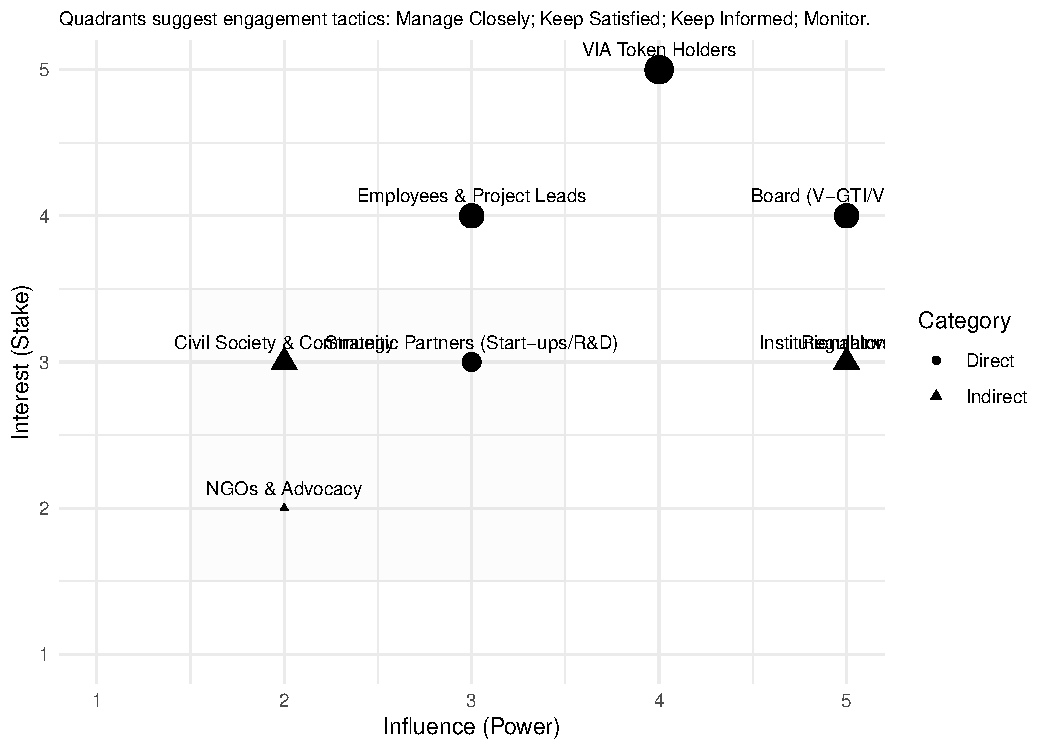
\includegraphics[keepaspectratio]{gp3_files/figure-pdf/stakeholder-map-viridis-1.pdf}}

}

\caption{VIRIDIS stakeholder map on a Power--Interest grid (1=low,
5=high).}

\end{figure}%

\begin{tcolorbox}[enhanced jigsaw, colframe=quarto-callout-tip-color-frame, coltitle=black, titlerule=0mm, opacitybacktitle=0.6, colback=white, toprule=.15mm, leftrule=.75mm, rightrule=.15mm, opacityback=0, toptitle=1mm, bottomtitle=1mm, bottomrule=.15mm, title=\textcolor{quarto-callout-tip-color}{\faLightbulb}\hspace{0.5em}{Tip}, arc=.35mm, left=2mm, colbacktitle=quarto-callout-tip-color!10!white, breakable]

Design implication. In a phased DAO rollout, Board and VIA token holders
belong in ``manage closely'' and should co-shape quorum, veto, and
escalation rules; Regulators and institutional investors require early
assurance and reporting pipelines; Employees/partners need structured
involvement channels (proposal authorship, advisory sprints) to prevent
token-only capture (\citeproc{ref-aghion1997-decentralization}{Aghion \&
Tirole, 1997}; \citeproc{ref-werner2020-governance-blockchain}{Werner et
al., 2020}).

\end{tcolorbox}

\subsection{Engagement Calibration (DAO--Enterprise
Hybrid)}\label{sec-stakeholders-engage}

Below, stakeholder groups are mapped to concrete engagement mechanisms
used later in governance design (see Chapters 6--9):

Empower (vote/submit) --- VIA token holders: proposal rights,
token-weighted voting, and transparent on-chain outcomes.

Collaborate (co-govern) --- Board; Strategic partners: hybrid
safeguards, joint working groups, and pre-enactment compliance checks.

Involve (co-design/advise) --- Employees \& project leads: scoped
authorship of proposals, sprint reviews, and change-impact feedback.

Consult (assure/align) --- Institutional investors; Regulators:
data-room access, taxonomy/SFDR-aligned dashboards, assurance briefings
(\citeproc{ref-european-commission-2019-financing-sustainable-growth}{Commission,
2019}; \citeproc{ref-kellers2022-mobilizing-capital}{Kellers, 2022}).

Inform (disclose/educate) --- Community, NGOs: quarterly transparency
reports and accessible summaries of decisions and impacts.

This calibrated map anchors the governance mechanisms to the realities
of power, interest, and legitimacy---reducing the classic gap between
``formal'' rules and how decisions are actually made in practice
(\citeproc{ref-aghion1997-decentralization}{Aghion \& Tirole, 1997};
\citeproc{ref-atzori2018-trust-chain}{Atzori, 2018}).

\section{Problem Statement: Governance and Investment
Gap}\label{sec-problem}

VIRIDIS faces a dual challenge that threatens both its immediate
survival and long-term growth:\\
1. \textbf{Insufficient investment} in its portfolio of green technology
projects.\\
2. \textbf{Outdated governance structure} that relies on a centralised,
hierarchical decision-making model.

The current governance setup concentrates authority in a small circle of
board members across V-GTI and V-ECO. While this structure provided
efficiency during the start-up phase, it now creates critical barriers:

\begin{itemize}
\tightlist
\item
  \textbf{Transparency Deficit}: Stakeholders outside the board have
  limited visibility into decision-making processes.\\
\item
  \textbf{Low Inclusivity}: Investors and community members lack
  meaningful influence, undermining engagement and trust.\\
\item
  \textbf{Slow Decision Cycles}: Bureaucratic bottlenecks hinder VIRIDIS
  from rapidly responding to opportunities in the dynamic sustainable
  finance sector.\\
\item
  \textbf{Investor Concerns}: Inadequate participatory mechanisms
  discourage capital inflows from both institutional and retail
  investors, who increasingly demand accountability and verifiable
  governance practices
  (\citeproc{ref-aghion1997-decentralization}{Aghion \& Tirole, 1997};
  \citeproc{ref-viridis2025-financial-report}{VIRIDIS, 2025a}).
\end{itemize}

Without reform, VIRIDIS risks failing to capture the fast-growing pool
of sustainable finance capital. The governance gap thus directly
intersects with the investment gap, creating a feedback loop: limited
trust reduces participation, which in turn limits growth capital,
further eroding credibility.

Relative to the incumbent board-centric model, the DAO-enabled design
moves formal and real authority closer to stakeholders, while preserving
compliance via hybrid safeguards.

\section{Opportunity in Sustainable Finance}\label{sec-opportunity}

The European Union's Green Deal and sustainable finance agenda highlight
the urgency of mobilising private capital to bridge the estimated
\textbf{€175--€290 billion annual investment gap} required to reach
climate neutrality by 2050
(\citeproc{ref-european-commission-2019-financing-sustainable-growth}{Commission,
2019}). Regulations such as the EU Taxonomy, SFDR, and new ESG
disclosure rules create strong incentives for transparent and
accountable investment practices.

For VIRIDIS, this landscape presents a unique opportunity:

\begin{itemize}
\tightlist
\item
  \textbf{Alignment with EU Policy}: By adopting decentralised,
  transparent governance systems, VIRIDIS can demonstrate compliance
  with sustainability disclosure requirements, positioning itself as a
  credible recipient of EU-aligned funding.\\
\item
  \textbf{Investor Attraction}: Capital markets and retail investors are
  actively searching for credible, verifiable green investments. A
  DAO-based model, with real-time dashboards and auditable decision
  records, meets these demands.\\
\item
  \textbf{First-Mover Advantage}: Few European green-tech investment
  firms have operationalised decentralised governance. By doing so,
  VIRIDIS can differentiate itself and build a reputation for
  transparency, accountability, and innovation.\\
\item
  \textbf{Network Effects}: Inclusive governance increases stakeholder
  participation, strengthening trust and expanding the ecosystem. This
  can generate positive feedback loops of engagement and investment.
\end{itemize}

In short, while governance inefficiencies are a barrier, they also
represent an opportunity: reforming governance can unlock capital flows,
enhance competitiveness, and align VIRIDIS with broader EU sustainable
finance transformations
(\citeproc{ref-kellers2022-mobilizing-capital}{Kellers, 2022};
\citeproc{ref-vonwachter2023-defi-phd}{Wachter, 2023}).

\begin{center}\rule{0.5\linewidth}{0.5pt}\end{center}

\section{Research Questions and Objectives}\label{sec-rq}

\subsection{Research Questions}\label{research-questions}

\begin{enumerate}
\def\labelenumi{\arabic{enumi}.}
\tightlist
\item
  \textbf{Investment Mobilisation}: Does a decentralised governance
  system outperform the current hierarchical model in attracting
  sustainable investment.\\
\item
  \textbf{Stakeholder Engagement}: Does inclusive decision-making
  stimulate higher levels of stakeholder participation across VIRIDIS
  projects, thereby strengthening network effects.\\
\item
  \textbf{Green Capital Allocation}: Does decentralised governance
  specifically channel more capital into \textbf{green technology
  investments} rather than general technology ventures.
\end{enumerate}

\subsection{Research Objectives}\label{research-objectives}

\begin{enumerate}
\def\labelenumi{\arabic{enumi}.}
\tightlist
\item
  Analyse the shortcomings of the current governance framework and
  identify critical transparency and participation gaps.\\
\item
  Evaluate decentralised governance designs (DAO models) in light of
  VIRIDIS's operational constraints and EU sustainable finance
  expectations.\\
\item
  Map and classify stakeholders to understand their incentives,
  salience, and preferred modes of engagement.\\
\item
  Prototype decentralised governance mechanisms (token-based voting,
  transparent dashboards, iterative feedback loops) and test them with
  direct and indirect stakeholders.\\
\item
  Construct a \textbf{multi-value business case} demonstrating financial
  viability, impact alignment, and strategic competitiveness.\\
\item
  Provide a phased \textbf{implementation roadmap} that enables VIRIDIS
  to transition toward decentralised governance while maintaining
  regulatory compliance and scalability.
\end{enumerate}

By addressing these questions and objectives, the research aims to
demonstrate how a carefully designed DAO-enabled governance system can
close both the governance and investment gaps, positioning VIRIDIS as a
frontrunner in sustainable innovation and finance.

\chapter{Context Analysis}\label{sec-context-analysis}

This chapter situates VIRIDIS within the external conditions that shape
feasible governance choices. It synthesises the EU's sustainable-finance
architecture (EU Taxonomy, SFDR, climate benchmarks) and the policy
logic behind them, then connects these to current thinking on platform
governance and decentralisation. The aim is to translate context into
design constraints and opportunities that will later inform solution
criteria and validation. In doing so, the chapter draws on EU sources
and governance scholarship that emphasise transparency, participation,
and auditable decision rights
(\citeproc{ref-aghion1997-decentralization}{Aghion \& Tirole, 1997};
\citeproc{ref-atzori2018-trust-chain}{Atzori, 2018};
\citeproc{ref-european-commission-2019-financing-sustainable-growth}{Commission,
2019}; \citeproc{ref-tkachuk2023-efficient-design}{Tkachuk, 2023};
\citeproc{ref-werner2020-governance-blockchain}{Werner et al., 2020}).

How the chapter is structured.

§2.1 distils the EU Green Deal's investment gap and disclosure logic,
framing why verifiable governance is a market requirement---not an
internal nicety.

§2.2 summarises industry trends toward programmable, decentralised
coordination and their institutional limits.

§2.3 benchmarks traditional vs.~decentralised governance to surface
testable design implications and KPIs.

§2.4 closes with a risk--opportunity lens that will be reused when
specifying safeguards and roll-out in later chapters.

\section{External Environment: EU Sustainable Finance and Green
Deal}\label{sec-eu}

The European Green Deal establishes a policy framework for achieving
climate neutrality by 2050. A critical component of this framework is
\textbf{sustainable finance}, which integrates environmental, social,
and governance (ESG) considerations into investment decisions. According
to the European Commission, Europe requires \textbf{€175--€290 billion
in additional yearly investment} to meet its 2030 and 2050 climate and
energy goals
(\citeproc{ref-european-commission-2019-financing-sustainable-growth}{Commission,
2019}).

Three flagship regulations shape the financial environment:\\
- \textbf{EU Taxonomy}: a classification system defining which economic
activities qualify as sustainable.\\
- \textbf{Sustainable Finance Disclosure Regulation (SFDR)}: obliges
financial institutions to disclose sustainability risks and impacts.\\
- \textbf{Climate Benchmarks and ESG Disclosures}: ensure comparability
and alignment with the Paris Agreement.

For VIRIDIS, this environment presents both constraints and
opportunities. Constraints arise from stricter compliance and reporting
demands. Opportunities lie in \textbf{capital flows redirected to
verifiable sustainable projects}, particularly those with transparent
governance and traceable impact.

\section{Industry Trends in Governance Models}\label{sec-trends}

Industry governance models are undergoing significant change due to
digital transformation and sustainability imperatives. Two overarching
trends stand out:

\begin{itemize}
\tightlist
\item
  \textbf{Platformisation}: Governance in digital platforms emphasises
  coordination, openness, and resource sharing. Blockchain-based
  platforms extend this by reducing reliance on intermediaries and
  shifting trust toward the protocol itself
  (\citeproc{ref-werner2020-governance-blockchain}{Werner et al.,
  2020}).\\
\item
  \textbf{Decentralisation}: Distributed ledger technologies enable
  \textbf{Decentralised Autonomous Organisations (DAOs)} that coordinate
  activities through transparent, programmable rules rather than
  hierarchical structures (\citeproc{ref-atzori2018-trust-chain}{Atzori,
  2018}).
\end{itemize}

\subsection{Cross-cutting Technical and Institutional
Trends}\label{sec-trends-cross}

\begin{enumerate}
\def\labelenumi{\arabic{enumi}.}
\tightlist
\item
  \textbf{Transparency and Traceability}: Regulators and investors
  demand verifiable reporting and auditable governance.\\
\item
  \textbf{Programmability and Automation}: Smart contracts allow rules
  to be enforced automatically, reducing administrative overhead.\\
\item
  \textbf{Stakeholder Inclusion}: Decentralised models encourage wider
  participation, improving legitimacy and resilience
  (\citeproc{ref-aghion1997-decentralization}{Aghion \& Tirole,
  1997}).\\
\item
  \textbf{Regulatory Alignment}: Adoption is shaped by EU disclosure
  requirements and ESG benchmarks.\\
\item
  \textbf{Institutional Experimentation}: Firms experiment with hybrid
  models combining traditional oversight with decentralised
  participation to balance compliance and innovation.
\end{enumerate}

\section{Benchmarking Traditional vs Decentralized
Governance}\label{sec-benchmark}

Traditional governance relies on hierarchical oversight, while
decentralised governance distributes authority across tokenised or
participatory systems. Benchmarking reveals fundamental differences:

\begin{longtable}[]{@{}
  >{\raggedright\arraybackslash}p{(\linewidth - 4\tabcolsep) * \real{0.2500}}
  >{\raggedright\arraybackslash}p{(\linewidth - 4\tabcolsep) * \real{0.3472}}
  >{\raggedright\arraybackslash}p{(\linewidth - 4\tabcolsep) * \real{0.4028}}@{}}
\caption{Benchmarking governance
models}\label{tbl-benchmark}\tabularnewline
\toprule\noalign{}
\begin{minipage}[b]{\linewidth}\raggedright
Dimension
\end{minipage} & \begin{minipage}[b]{\linewidth}\raggedright
Traditional Governance
\end{minipage} & \begin{minipage}[b]{\linewidth}\raggedright
Decentralised Governance
\end{minipage} \\
\midrule\noalign{}
\endfirsthead
\toprule\noalign{}
\begin{minipage}[b]{\linewidth}\raggedright
Dimension
\end{minipage} & \begin{minipage}[b]{\linewidth}\raggedright
Traditional Governance
\end{minipage} & \begin{minipage}[b]{\linewidth}\raggedright
Decentralised Governance
\end{minipage} \\
\midrule\noalign{}
\endhead
\bottomrule\noalign{}
\endlastfoot
Decision-making & Centralised, board-driven & Distributed, token- or
member-driven \\
Transparency & Periodic reports & Continuous, on-chain data \\
Participation & Limited to executives/board & Open to wider stakeholder
groups \\
Accountability & Opaque, delayed & Traceable, auditable in real time \\
Adaptability & Slow, reactive & Flexible, programmable \\
\end{longtable}

\subsection{Design Implications for VIRIDIS}\label{sec-implications}

\begin{itemize}
\tightlist
\item
  VIRIDIS must shorten decision cycles to compete in fast-moving green
  tech markets.\\
\item
  Transparent dashboards and voting mechanisms would directly align with
  EU disclosure rules.\\
\item
  Tokenisation could serve a dual purpose of mobilising capital and
  granting governance rights.\\
\item
  Inclusive governance strengthens trust and broadens the investor base.
\end{itemize}

\subsection{Key Performance Indicators for Evaluation}\label{sec-kpis}

\begin{itemize}
\tightlist
\item
  \textbf{Participation Rate}: \% of stakeholders actively involved in
  decision-making.\\
\item
  \textbf{Capital Inflow}: additional investment raised under
  decentralised governance.\\
\item
  \textbf{Decision Cycle Time}: average time to move from proposal to
  decision.\\
\item
  \textbf{Transparency Index}: proportion of governance events publicly
  auditable.\\
\item
  \textbf{Trust Indicators}: survey-based metrics of investor and
  stakeholder confidence.
\end{itemize}

\section{Risks and Opportunities in Transition}\label{sec-risks}

\textbf{Risks}\\
- \textbf{Technical}: vulnerabilities in smart contracts or blockchain
scalability (\citeproc{ref-tkachuk2023-efficient-design}{Tkachuk,
2023}).\\
- \textbf{Cultural}: resistance among employees or investors unfamiliar
with decentralised processes.\\
- \textbf{Regulatory}: unclear status of DAOs within EU financial
regulation creates compliance uncertainty.

\textbf{Opportunities}\\
- \textbf{Capital Mobilisation}: alignment with EU sustainable finance
frameworks positions VIRIDIS as a credible investment destination
(\citeproc{ref-kellers2022-mobilizing-capital}{Kellers, 2022}).\\
- \textbf{Innovation}: decentralised governance fosters rapid
experimentation and idea generation.\\
- \textbf{Competitive Differentiation}: by adopting DAO principles,
VIRIDIS can establish itself as a frontrunner in sustainable finance and
governance innovation.

\chapter{Scope and Limitations}\label{sec-scope}

This chapter makes the study operational: it defines what is inside
scope (analysis and design of a DAO-enabled governance model for
VIRIDIS), what is explicitly excluded (full production build and legal
adjudication), and what limitations shape interpretation (single-case
design, time-bounded data, prototype fidelity). The intent is to balance
ambition with academic discipline, ensuring that findings are credible,
replicable, and actionable within the project window.

How the chapter is structured.

§3.1 articulates scope with clear deliverables (analysis → design →
prototype evidence → business case → roadmap).

§3.2 lists exclusions to avoid scope creep while preserving
decision-useful outputs for implementation.

§3.3 states limitations (internal/external validity risks) and explains
why results still provide a sound basis for solution development and GP4
execution.

\section{Scope of the Project}\label{sec-in}

The scope of this project is the \textbf{design, analysis, and
validation} of a decentralised governance model for VIRIDIS. The project
specifically focuses on how governance reform can support capital
mobilisation and improve stakeholder participation within the company's
sustainable finance ecosystem.

The work includes:\\
- A comprehensive analysis of the \textbf{current governance structure}
of VIRIDIS.\\
- A \textbf{stakeholder mapping and classification} to identify
incentives and engagement mechanisms.\\
- The application of ideation and design methods (SCAMPER, heatmaps,
iteration rounds) to generate solution concepts.\\
- The \textbf{design of a DAO-enabled operating model}, including
token-based voting, transparent dashboards, and rule-setting
mechanisms.\\
- Testing through \textbf{prototyping, workshops, and feedback loops}
with both direct and indirect stakeholders.\\
- Development of a \textbf{multi-value business case} that covers
financial, technological, and societal dimensions.\\
- A \textbf{phased implementation roadmap} aligned with EU sustainable
finance frameworks and VIRIDIS's growth strategy.

\section{Out of Scope}\label{sec-out}

Several areas fall outside the scope of this report to maintain focus
and feasibility:

\begin{itemize}
\tightlist
\item
  \textbf{Full-scale technical implementation}: while prototypes are
  developed, a production-ready blockchain infrastructure is outside the
  scope.\\
\item
  \textbf{Policy design beyond EU frameworks}: global regulatory
  harmonisation is acknowledged but not addressed in detail.\\
\item
  \textbf{Non-financial performance of portfolio startups}: the emphasis
  is on governance and capital mobilisation rather than sectoral
  technology outcomes.\\
\item
  \textbf{Long-term macroeconomic forecasting}: while scenarios are
  explored, full predictive modelling of global markets is excluded.\\
\item
  \textbf{Legal adjudication}: the report does not provide binding legal
  interpretations of DAO or token regulation.
\end{itemize}

\section{Limitations}\label{sec-limits}

This study is subject to several limitations:

\begin{itemize}
\tightlist
\item
  \textbf{Single-case design}: focusing on VIRIDIS limits
  generalisability to other firms, though findings may have broader
  relevance.\\
\item
  \textbf{Time-bound research}: the report is based on a one-year
  project window, restricting longitudinal analysis of governance
  impacts.\\
\item
  \textbf{Stakeholder sampling}: while both direct and indirect
  stakeholders were consulted, the number of participants was
  constrained by availability and project scope.\\
\item
  \textbf{Prototype fidelity}: prototypes used in workshops are
  simplified representations and may not capture all technical
  complexities of DAO systems.\\
\item
  \textbf{Regulatory uncertainty}: EU frameworks are evolving, meaning
  that assumptions made in this study could shift as new laws and
  guidelines are introduced.
\end{itemize}

Despite these limitations, the study provides a robust foundation for
evaluating the viability of decentralised governance at VIRIDIS and for
informing further development.

\chapter{Problem Analysis and Research}\label{sec-analysis}

Chapter 4 turns inward. It analyses VIRIDIS's current governance reality
and traces how structural choices produce real authority outcomes for
stakeholders---sometimes at odds with formal intent
(\citeproc{ref-aghion1997-decentralization}{Aghion \& Tirole, 1997}).
The analysis integrates document review, stakeholder inputs, and
prototype feedback to identify where and why transparency, inclusion,
and decision speed break down. It also considers technological readiness
and constraints highlighted in decentralised governance research
(\citeproc{ref-atzori2018-trust-chain}{Atzori, 2018};
\citeproc{ref-tkachuk2023-efficient-design}{Tkachuk, 2023}).

How the chapter is structured.

§4.1 maps today's oversight, culture, and infrastructure and explains
their investor-relevant consequences, referencing internal materials
where appropriate (\citeproc{ref-viridis2025-financial-report}{VIRIDIS,
2025a}).

§4.2 consolidates the diagnosed gaps---decision-making, transparency,
inclusion---into design requirements that directly feed the solution
criteria in Chapter (\citeproc{ref-ref}{\textbf{ref?}})(sec-ideation)
and the architecture in Chapter
(\citeproc{ref-ref}{\textbf{ref?}})(sec-arch).

\section{Current Governance Setup}\label{sec-current-gov}

VIRIDIS currently employs a \textbf{dual-entity governance structure}:\\
- \textbf{V-GTI (VIRIDIS Green Tech Investment AG)} is the for-profit
entity responsible for raising capital, managing investments, and
steering strategic decision-making.\\
- \textbf{V-ECO (VIRIDIS Eco-System gGmbH)} is the non-profit branch
focused on incubation, education, and community engagement.

While this structure reflects the company's hybrid mission of generating
both economic and social value, it suffers from several inefficiencies:
overlapping board membership, centralisation of authority, and lack of
transparent communication with broader stakeholders. These issues have a
direct impact on investor confidence, stakeholder trust, and overall
scalability.

\subsection{Structure and Oversight}\label{sec-oversight}

The oversight system is highly centralised, with decision-making
concentrated in the boards of V-GTI and V-ECO. Key characteristics
include:

\begin{itemize}
\tightlist
\item
  \textbf{Board Overlap}: Many directors sit on both boards, reducing
  diversity of perspectives and concentrating power.\\
\item
  \textbf{Hierarchical Decision Flow}: Strategic initiatives require
  approval from a small executive group, delaying responsiveness.\\
\item
  \textbf{Accountability Gaps}: Oversight mechanisms are internally
  managed, limiting external visibility into governance outcomes.
\end{itemize}

This structural design ensures control but weakens inclusivity. For a
firm competing in the sustainable finance domain, where transparency and
participation are critical, the current model undermines alignment with
investor and regulatory expectations.

\subsection{Talent and Culture}\label{sec-culture}

The cultural environment within VIRIDIS is shaped by its early-stage
entrepreneurial context. The team demonstrates strong \textbf{commitment
to sustainability and innovation}, yet several challenges have been
identified:

\begin{itemize}
\tightlist
\item
  \textbf{Centralised Decision Culture}: Employees and mid-level
  managers have limited input into strategic choices, which reduces
  engagement and slows innovation.\\
\item
  \textbf{Participation Barriers}: Community members and token investors
  lack clear mechanisms to contribute ideas or influence governance.\\
\item
  \textbf{Trust Deficit}: Stakeholder interviews conducted during GP2
  revealed concerns about transparency and inclusivity, particularly
  among external partners and investors.
\end{itemize}

A decentralised governance system could help shift this culture toward
one of \textbf{shared ownership, accountability, and innovation},
thereby increasing both trust and productivity.

\subsection{Infrastructure and Technology}\label{sec-it}

The current technological infrastructure of VIRIDIS supports core
operations but lacks integrated systems for decentralised participation.
Identified issues include:

\begin{itemize}
\tightlist
\item
  \textbf{Fragmented IT Systems}: Governance and investment processes
  are supported by traditional digital tools but not by
  blockchain-enabled platforms.\\
\item
  \textbf{Limited Transparency Tools}: Reporting is largely periodic and
  static, falling short of the real-time traceability expected by
  sustainable finance stakeholders.\\
\item
  \textbf{No On-Chain Governance}: The VIA Security Token exists
  primarily as a financial instrument; its governance functionalities
  (e.g., voting rights) are not fully operationalised.
\end{itemize}

These limitations highlight the need for a \textbf{blockchain-based
governance infrastructure} with features such as:\\
- Token-weighted voting.\\
- Smart contract--based rules and accountability.\\
- Dashboards for real-time transparency and monitoring.

Together, these reforms can transform the VIRIDIS governance model into
one that aligns with EU regulatory expectations and investor preferences
for transparent, auditable systems.

\section{Assessment of Gaps in Decision-Making and
Inclusion}\label{sec-gaps}

The assessment of governance practices at VIRIDIS reveals a set of
critical gaps in decision-making and inclusion. These gaps directly
undermine the firm's ability to mobilise capital, build trust, and align
with sustainable finance expectations.

\subsection{Hierarchical Limitations}\label{sec-hier}

The current governance structure is hierarchical and centralised, with
most decision-making power concentrated at the executive and board
levels. This creates several problems:

\begin{itemize}
\tightlist
\item
  \textbf{Bureaucratic Bottlenecks}: Decisions require multiple layers
  of approval, leading to delays in fast-moving markets.\\
\item
  \textbf{Concentration of Authority}: A small circle of board members
  holds disproportionate influence, reducing diversity of
  perspectives.\\
\item
  \textbf{Low Stakeholder Agency}: Employees, token investors, and
  community members have limited or no role in shaping strategic
  initiatives.
\end{itemize}

These limitations restrict VIRIDIS's responsiveness to emerging
opportunities in the green-tech sector and diminish the inclusivity
needed for stakeholder trust.

\subsection{Transparency and Communication Gaps}\label{sec-comm}

A consistent theme from stakeholder feedback is the lack of transparency
in governance processes. Identified gaps include:

\begin{itemize}
\tightlist
\item
  \textbf{Opaque Decision Processes}: Stakeholders outside the board
  cannot trace how or why strategic decisions are made.\\
\item
  \textbf{Irregular Communication}: Reporting is periodic and often
  delayed, limiting the availability of up-to-date information.\\
\item
  \textbf{Perceived Exclusion}: Investors and community members perceive
  governance as a closed process, which discourages engagement and
  weakens credibility.
\end{itemize}

This gap contrasts sharply with EU sustainable finance regulations,
which demand auditable and verifiable disclosures. Without improvement,
VIRIDIS risks failing to meet both regulatory requirements and investor
expectations.

\subsection{Technology Adoption Challenges}\label{sec-tech-chal}

Although VIRIDIS has introduced the VIA Security Token,
governance-related technology adoption remains incomplete. Key
challenges include:

\begin{itemize}
\tightlist
\item
  \textbf{Underutilised Token Functionality}: VIA is primarily used as a
  financial instrument; its governance potential (voting rights,
  proposal systems) has not been fully activated.\\
\item
  \textbf{Lack of Integrated Dashboards}: No unified platform exists to
  display governance events, voting outcomes, or project progress in
  real time.\\
\item
  \textbf{Limited Experimentation}: Prototypes for decentralised tools
  are still in early testing stages, preventing broader adoption and
  learning.
\end{itemize}

The absence of robust technological infrastructure prevents the company
from operationalising decentralised governance and realising its
benefits. As a result, investor trust, stakeholder participation, and
regulatory alignment remain below potential.

\textbf{Summary}\\
The combined effect of hierarchical limitations, transparency deficits,
and incomplete technology adoption creates a governance gap that
directly constrains investment mobilisation. Addressing these gaps
through decentralised, DAO-enabled governance mechanisms is essential
for VIRIDIS to achieve credibility, scalability, and alignment with EU
sustainable finance frameworks.

\chapter{Stakeholder Analysis, Mapping, and
Engagement}\label{sec-engagement}

Decentralised governance only works if it engages the actors who
actually hold power, legitimacy, or critical knowledge. This chapter
identifies VIRIDIS's direct and indirect stakeholders, maps them on a
power--interest grid, and calibrates engagement modes (inform, consult,
involve, collaborate, empower) appropriate for a DAO--enterprise hybrid.
The goal is a practical participation blueprint that is both politically
realistic and aligned with transparency norms in sustainable finance
(\citeproc{ref-atzori2018-trust-chain}{Atzori, 2018};
\citeproc{ref-european-commission-2019-financing-sustainable-growth}{Commission,
2019}; \citeproc{ref-werner2020-governance-blockchain}{Werner et al.,
2020}).

How the chapter is structured.

§5.1--§5.2 define the stakeholder set and present the mapping (tabular
and visual).

§5.3 aligns groups to engagement mechanisms that later become concrete
rules and interfaces in Chapter

§5.4 summarises adoption scenarios to anticipate change dynamics and
inform the phased roll-out strategy in Chapter

\section{Identification of Key Stakeholders}\label{sec-ident}

The VIRIDIS ecosystem brings together a diverse set of stakeholders,
both internal and external, who influence and are affected by governance
outcomes. Based on interviews, document analysis, and workshop data, the
following groups are identified:

\begin{itemize}
\tightlist
\item
  \textbf{Internal Stakeholders}

  \begin{itemize}
  \tightlist
  \item
    Board of Directors (V-GTI, V-ECO)\\
  \item
    Employees and project managers\\
  \item
    Token investors (VIA holders)
  \end{itemize}
\item
  \textbf{External Stakeholders}

  \begin{itemize}
  \tightlist
  \item
    Strategic partners (start-ups, incubated ventures, R\&D
    institutions)\\
  \item
    Government and regulatory bodies (EU financial authorities,
    sustainability regulators)\\
  \item
    Community participants (local initiatives, civil society actors,
    sustainability advocates)\\
  \item
    Private and institutional investors
  \end{itemize}
\end{itemize}

\section{Stakeholder Mapping (Direct and Indirect)}\label{sec-map}

Stakeholders are categorised as \textbf{direct} (actively involved in
governance or operations) or \textbf{indirect} (influenced by governance
decisions but not directly participating).

\begin{longtable}[]{@{}
  >{\raggedright\arraybackslash}p{(\linewidth - 4\tabcolsep) * \real{0.2466}}
  >{\raggedright\arraybackslash}p{(\linewidth - 4\tabcolsep) * \real{0.4384}}
  >{\raggedright\arraybackslash}p{(\linewidth - 4\tabcolsep) * \real{0.3151}}@{}}
\caption{Direct and indirect stakeholder
mapping}\label{tbl-stakeholders}\tabularnewline
\toprule\noalign{}
\begin{minipage}[b]{\linewidth}\raggedright
Category
\end{minipage} & \begin{minipage}[b]{\linewidth}\raggedright
Stakeholder Group
\end{minipage} & \begin{minipage}[b]{\linewidth}\raggedright
Role in Governance
\end{minipage} \\
\midrule\noalign{}
\endfirsthead
\toprule\noalign{}
\begin{minipage}[b]{\linewidth}\raggedright
Category
\end{minipage} & \begin{minipage}[b]{\linewidth}\raggedright
Stakeholder Group
\end{minipage} & \begin{minipage}[b]{\linewidth}\raggedright
Role in Governance
\end{minipage} \\
\midrule\noalign{}
\endhead
\bottomrule\noalign{}
\endlastfoot
Direct & Board of Directors (V-GTI, V-ECO) & Strategic oversight,
approval \\
Direct & Employees and managers & Project execution \\
Direct & VIA token holders & Financial participation, voting \\
Direct & Strategic partners (start-ups, R\&D) & Joint ventures,
co-governance \\
Indirect & Government and regulators & Compliance, policy shaping \\
Indirect & Civil society and community groups & Legitimacy, social
licence \\
Indirect & Institutional investors & Capital mobilisation \\
\end{longtable}

\section{Engagement Levels and Classifications}\label{sec-engage-levels}

Each stakeholder group is assigned an engagement strategy, drawing on
the IAP2 framework (inform, consult, involve, collaborate, empower):

\begin{itemize}
\tightlist
\item
  \textbf{Inform}: Regulators and government bodies (transparent
  reporting, compliance updates).\\
\item
  \textbf{Consult}: Institutional investors (feedback on governance, ESG
  alignment).\\
\item
  \textbf{Involve}: Employees and project managers (participation in
  workshops, advisory roles).\\
\item
  \textbf{Collaborate}: Strategic partners and start-ups (joint
  governance initiatives, co-design).\\
\item
  \textbf{Empower}: Token holders and community participants (voting
  rights, proposal mechanisms).
\end{itemize}

This classification ensures that participation mechanisms are calibrated
to the influence, interest, and salience of each stakeholder group.

\section{Multi-Perspective Change Scenarios}\label{sec-scenarios}

To anticipate governance reforms, VIRIDIS explored multi-perspective
change scenarios with stakeholders. Three key scenarios emerged:

\begin{enumerate}
\def\labelenumi{\arabic{enumi}.}
\tightlist
\item
  \textbf{Incremental Reform (Hybrid Model)}

  \begin{itemize}
  \tightlist
  \item
    Retains hierarchical oversight but introduces consultative
    mechanisms for token holders and employees.\\
  \item
    Low risk, but limited transformative impact on transparency and
    trust.
  \end{itemize}
\item
  \textbf{Participatory DAO (Phased Rollout)}

  \begin{itemize}
  \tightlist
  \item
    Gradually expands decision-making rights to token holders and
    community members.\\
  \item
    Uses pilots and prototypes to test dashboards, voting, and proposal
    systems.\\
  \item
    Balances compliance with inclusivity.
  \end{itemize}
\item
  \textbf{Full DAO Transition}

  \begin{itemize}
  \tightlist
  \item
    Transfers significant decision rights to a decentralised governance
    system.\\
  \item
    Maximises transparency, accountability, and stakeholder inclusion.\\
  \item
    Carries higher regulatory and cultural risks, but also greater
    potential for differentiation and innovation.
  \end{itemize}
\end{enumerate}

These scenarios reflect the range of possible pathways for VIRIDIS, from
cautious adaptation to bold transformation. Stakeholder input
consistently emphasised the importance of a \textbf{phased approach},
starting with hybrid models and scaling toward decentralised governance
as trust and capability grow.

\chapter{Solution Design and Development}\label{sec-solution}

The solution emerged via a multi-round design process (mapping →
ideation → heatmap → prototyping → validation) with direct and indirect
stakeholders (see §7), meeting the `Approach' criterion.

\section{Gap Analysis from GP3 Research}\label{sec-gap-res}

The findings from GP3 research highlight three central governance gaps
at VIRIDIS:

\begin{itemize}
\tightlist
\item
  \textbf{Decision-Making}: Overly centralised authority restricts
  agility and responsiveness.\\
\item
  \textbf{Transparency}: Lack of real-time reporting and limited
  stakeholder visibility reduce trust.\\
\item
  \textbf{Inclusion}: Investors, employees, and community members have
  insufficient voice in shaping strategy.
\end{itemize}

Workshops and interviews confirmed that these gaps translate into lower
participation rates, weak investor confidence, and limited capital
inflow. Addressing them requires an operating model that distributes
authority, leverages technology for transparency, and expands
participation beyond the board level.

\begin{center}\rule{0.5\linewidth}{0.5pt}\end{center}

\section{Ideation Process and Design Criteria}\label{sec-ideation}

The ideation process applied a structured design-thinking approach
supported by the SCAMPER framework. Stakeholders were invited to
co-create solutions through workshops and brainstorming sessions. Three
design criteria guided the process:

\begin{enumerate}
\def\labelenumi{\arabic{enumi}.}
\tightlist
\item
  \textbf{Inclusivity}: Broaden participation by embedding mechanisms
  for token holders, employees, and partners.\\
\item
  \textbf{Transparency}: Provide real-time, verifiable reporting of
  decisions and outcomes.\\
\item
  \textbf{Feasibility}: Ensure proposed solutions are technically
  implementable and align with EU regulatory frameworks.
\end{enumerate}

\subsection{Iteration Round 1: Idea Generation}\label{sec-it1}

In the first ideation round, participants generated a broad set of
potential solutions. Key ideas included:

\begin{itemize}
\tightlist
\item
  \textbf{Token-weighted voting} using the VIA Security Token.\\
\item
  \textbf{Transparent dashboards} displaying governance events and
  financial flows.\\
\item
  \textbf{Delegated voting mechanisms} to increase efficiency while
  maintaining inclusivity.\\
\item
  \textbf{Smart contract--based rules} for automatic execution of
  governance decisions.\\
\item
  \textbf{Hybrid governance models} combining DAO participation with
  board oversight.
\end{itemize}

\begin{figure}

\centering{

\pandocbounded{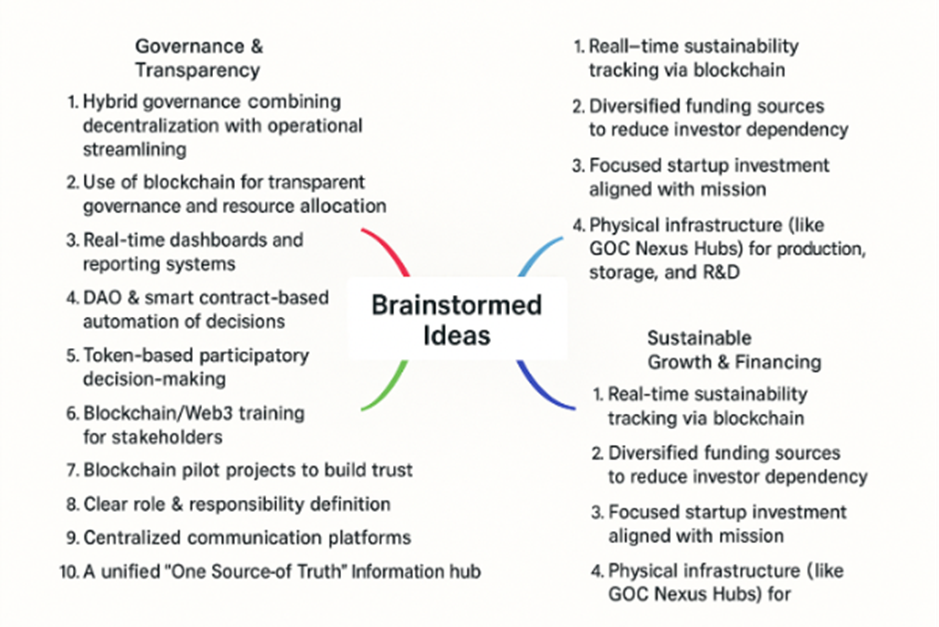
\includegraphics[keepaspectratio]{figs/BrainstormedIdeas.png}}

}

\caption{\label{fig-brainstorm}}

\end{figure}%

These ideas provided the foundation for subsequent evaluation and
prioritisation.

\subsection{Heatmap Analysis and Ratings}\label{sec-heatmap}

To evaluate the feasibility and impact of the brainstormed ideas, a
heatmap analysis was conducted. Stakeholders rated each idea across
three dimensions:

\begin{itemize}
\tightlist
\item
  \textbf{Impact}: Potential to improve participation, trust, and
  capital mobilisation.\\
\item
  \textbf{Feasibility}: Technical and organisational implementability in
  the short-to-medium term.\\
\item
  \textbf{Alignment}: Fit with EU sustainable finance frameworks and
  VIRIDIS strategy.
\end{itemize}

\begin{longtable}[]{@{}
  >{\raggedright\arraybackslash}p{(\linewidth - 8\tabcolsep) * \real{0.3816}}
  >{\centering\arraybackslash}p{(\linewidth - 8\tabcolsep) * \real{0.1053}}
  >{\centering\arraybackslash}p{(\linewidth - 8\tabcolsep) * \real{0.1711}}
  >{\centering\arraybackslash}p{(\linewidth - 8\tabcolsep) * \real{0.1447}}
  >{\centering\arraybackslash}p{(\linewidth - 8\tabcolsep) * \real{0.1974}}@{}}
\caption{Heatmap analysis of governance design
ideas}\label{tbl-heatmap}\tabularnewline
\toprule\noalign{}
\begin{minipage}[b]{\linewidth}\raggedright
Idea
\end{minipage} & \begin{minipage}[b]{\linewidth}\centering
Impact
\end{minipage} & \begin{minipage}[b]{\linewidth}\centering
Feasibility
\end{minipage} & \begin{minipage}[b]{\linewidth}\centering
Alignment
\end{minipage} & \begin{minipage}[b]{\linewidth}\centering
Overall Score
\end{minipage} \\
\midrule\noalign{}
\endfirsthead
\toprule\noalign{}
\begin{minipage}[b]{\linewidth}\raggedright
Idea
\end{minipage} & \begin{minipage}[b]{\linewidth}\centering
Impact
\end{minipage} & \begin{minipage}[b]{\linewidth}\centering
Feasibility
\end{minipage} & \begin{minipage}[b]{\linewidth}\centering
Alignment
\end{minipage} & \begin{minipage}[b]{\linewidth}\centering
Overall Score
\end{minipage} \\
\midrule\noalign{}
\endhead
\bottomrule\noalign{}
\endlastfoot
Token-weighted voting & High & Medium & High & 8.5 \\
Transparent dashboards & High & High & High & 9.0 \\
Delegated voting & Medium & Medium & Medium & 6.5 \\
Smart contract rules & High & Medium & High & 8.0 \\
Hybrid DAO-board governance & Medium & High & High & 8.0 \\
\end{longtable}

The results indicate that \textbf{transparent dashboards} and
\textbf{token-weighted voting} emerged as the most impactful and
feasible starting points. Smart contract rules and hybrid governance
models were also prioritised for phased implementation, while delegated
voting was considered less urgent.

\subsection{Iteration Round 2}\label{sec-it2}

In the second iteration, the shortlisted ideas from the heatmap were
refined with stakeholder feedback. Prototypes of dashboards and mock-ups
of voting flows were presented in workshops. Key developments included:

\begin{itemize}
\tightlist
\item
  \textbf{Dashboard Prototype}: A visual interface showing proposals,
  voting outcomes, and financial flows in real time.\\
\item
  \textbf{Voting Flow Simulation}: Token holders simulated casting votes
  on pilot decisions using mock tokens.\\
\item
  \textbf{Risk Mitigation Discussions}: Stakeholders raised concerns
  about regulatory compliance, prompting the addition of oversight
  features.
\end{itemize}

Stakeholder ratings in this round confirmed the need for a phased
rollout, beginning with dashboards and voting, followed by more advanced
smart contract automation.

\subsection{Iteration Round 3: Final Selection}\label{sec-it3}

The third iteration focused on consolidation. Participants compared
refined solutions and voted on the final design package. The following
elements were selected:

\begin{itemize}
\tightlist
\item
  \textbf{Core Features}:

  \begin{itemize}
  \tightlist
  \item
    Token-weighted voting (VIA Security Token).\\
  \item
    Transparent dashboards for proposals and outcomes.\\
  \item
    Governance rules embedded in smart contracts for accountability.
  \end{itemize}
\item
  \textbf{Supporting Features}:

  \begin{itemize}
  \tightlist
  \item
    Delegated voting as an optional efficiency tool.\\
  \item
    Hybrid oversight to balance board authority with DAO participation.
  \end{itemize}
\end{itemize}

\section{Optimal Innovation Solution}\label{sec-optimal}

The optimal solution is a \textbf{DAO-enabled governance model} that
integrates decentralised participation with transparent oversight
mechanisms. Its key characteristics include:

\begin{itemize}
\tightlist
\item
  \textbf{Inclusive Participation}: All VIA token holders can vote on
  strategic proposals.\\
\item
  \textbf{Transparency}: Real-time dashboards display proposals, voting
  outcomes, and financial allocations.\\
\item
  \textbf{Programmability}: Smart contracts enforce governance rules
  automatically, reducing manipulation risk.\\
\item
  \textbf{Hybrid Oversight}: The board retains a supervisory role,
  ensuring compliance with EU regulations.
\end{itemize}

This solution directly addresses VIRIDIS's governance gaps by broadening
stakeholder engagement, increasing transparency, and mobilising
investment capital.

\begin{figure}

\centering{

\pandocbounded{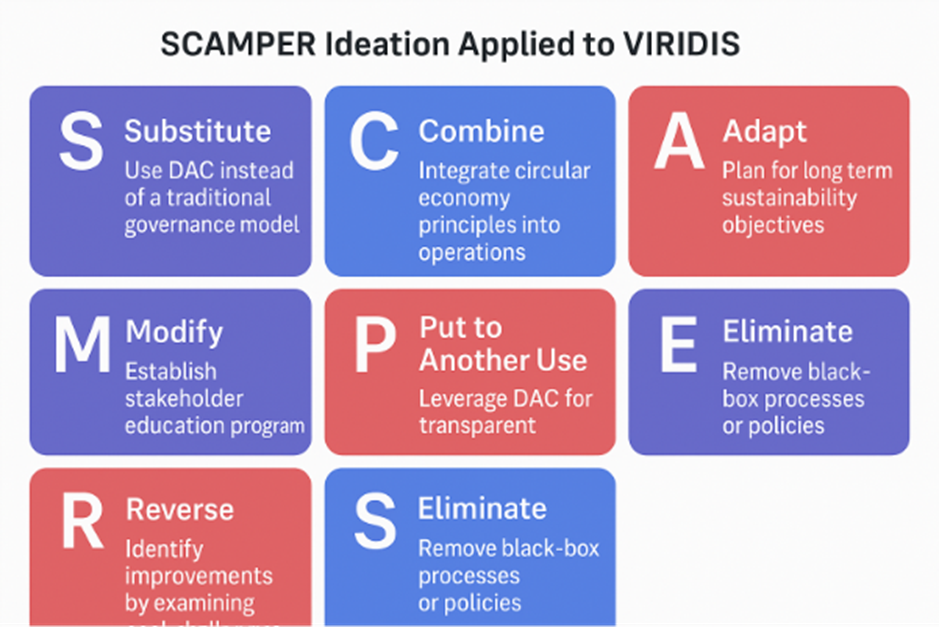
\includegraphics[keepaspectratio]{figs/Viridis Governance Operating Model.png}}

}

\caption{\label{fig-viridis-model}}

\end{figure}%

\section{Governance Architecture Overview}\label{sec-arch}

The governance design is specified at \textbf{architecture level} (what
must exist), not at \textbf{implementation level} (how it will be
built). This keeps GP3 within scope while making GP4 executable.

\textbf{Core components}

\begin{itemize}
\item
  \textbf{Voting layer (VIA-based)}\\
  Token-weighted ballots with quorum and majority thresholds.
  Categories: strategic portfolio choices, sustainability initiatives,
  and community programs. Advisory by default; categories and thresholds
  are codified in the rule set.
\item
  \textbf{Rules \& policy layer}\\
  A canonical ruleset defines (i) proposal lifecycle, (ii) eligibility,
  (iii) conflict-of-interest handling, and (iv) escalation paths. Edge
  cases (ties, lapsed quorums, urgent votes) are pre-defined to avoid
  ambiguity.
\item
  \textbf{Transparency layer (governance dashboard spec)}\\
  Public-by-default views of proposals, live vote tallies, outcomes, and
  post-decision actions. An audit pane shows immutable decision logs
  mapped to EU ESG disclosure items (taxonomy objective, DNSH, minimum
  safeguards).
\item
  \textbf{Oversight \& safeguards}\\
  A supervisory check ensures legal and compliance alignment prior to
  enactment. Any exception path is time-boxed and logged to preserve
  accountability.
\item
  \textbf{Data model (minimal)}\\
  \texttt{Proposal(id,\ category,\ sponsor,\ created\_at,\ closes\_at,\ esg\_tags)}\strut \\
  \texttt{Ballot(id,\ proposal\_id,\ voter\_id,\ weight,\ cast\_at)}\strut \\
  \texttt{Outcome(proposal\_id,\ quorum,\ result,\ enacted\_at,\ reference\_link)}
\end{itemize}

\subsection{Technical Design (Voting, Token, Dashboard)}\label{sec-tech}

The technical implementation plan builds on three modules:

\begin{enumerate}
\def\labelenumi{\arabic{enumi}.}
\tightlist
\item
  \textbf{Voting Mechanism}: Token-weighted voting integrated into the
  VIA Security Token smart contract.\\
\item
  \textbf{Governance Dashboard}: Web-based interface showing proposals,
  votes, and outcomes.\\
\item
  \textbf{Smart Contracts}: Automated enforcement of governance rules,
  including quorum thresholds and veto options.
\end{enumerate}

The system is designed for gradual rollout, starting with advisory votes
before moving to binding governance decisions.

\subsection{Governance Structure and Rules}\label{sec-structure}

The governance framework defines responsibilities and safeguards:

\begin{itemize}
\tightlist
\item
  \textbf{Proposal Submission}: Token holders and board members can
  submit proposals.\\
\item
  \textbf{Voting Rules}: Decisions require quorum and majority
  thresholds defined in smart contracts.\\
\item
  \textbf{Delegated Voting}: Optional mechanism for efficiency, allowing
  token holders to delegate votes.\\
\item
  \textbf{Oversight Layer}: The board retains veto power over proposals
  that conflict with legal or regulatory requirements.\\
\item
  \textbf{Audit and Traceability}: All actions are logged on-chain for
  transparency and accountability.
\end{itemize}

This structure balances decentralisation with the compliance and
stability required by EU regulators.

\section{Implications for VIRIDIS}\label{sec-implications-viridis}

Adopting this DAO-enabled governance model has several implications:

\begin{itemize}
\tightlist
\item
  \textbf{Strategic}: Positions VIRIDIS as a pioneer in sustainable
  finance governance, differentiating it in the European market.\\
\item
  \textbf{Financial}: Enhanced transparency and inclusion increase
  investor confidence, mobilising additional capital flows.\\
\item
  \textbf{Cultural}: Shifts organisational culture toward participation,
  accountability, and innovation.\\
\item
  \textbf{Regulatory}: Aligns governance practices with EU disclosure
  frameworks while retaining oversight mechanisms to mitigate legal
  uncertainty.\\
\item
  \textbf{Scalability}: Creates a governance infrastructure capable of
  growing with VIRIDIS's ecosystem, supporting future expansion into
  global markets.
\end{itemize}

The transition to this model requires careful implementation but offers
transformative potential in addressing both the governance and
investment gaps at VIRIDIS.

\chapter{Validation and Testing}\label{sec-validation}

This chapter evidences the working prototype (governance dashboard mock
+ token-voting flow) and the workshops used for validation; these are
the artefacts required under GP3 (solution + prototype + validation)

\section{Prototyping (Dashboard, Token Voting
Flow)}\label{sec-prototype}

Prototypes were developed to test the functionality and usability of
decentralised governance tools. Two main prototypes were created:

\begin{itemize}
\tightlist
\item
  \textbf{Governance Dashboard}: A web interface displaying proposals,
  live voting outcomes, and project metrics.\\
\item
  \textbf{Token Voting Flow}: A simulation of VIA Security Token--based
  voting, allowing participants to cast votes and see results reflected
  on the dashboard.
\end{itemize}

These prototypes demonstrated the feasibility of integrating
blockchain-based decision-making with user-friendly interfaces.

\section{Pilot Workshops and Feedback Loops}\label{sec-workshops}

Pilot workshops were conducted with selected employees, token holders,
and partners. Participants interacted with the prototypes and provided
feedback on:

\begin{itemize}
\tightlist
\item
  \textbf{Usability}: Interface clarity, ease of navigation, and voting
  mechanics.\\
\item
  \textbf{Trust}: Perceived transparency of decision-making processes.\\
\item
  \textbf{Functionality}: Adequacy of reporting features and proposal
  tracking.
\end{itemize}

Feedback loops were integrated by iteratively refining the prototypes
after each workshop session. This ensured progressive improvement and
alignment with stakeholder expectations.

\section{Validation with Direct Stakeholders}\label{sec-direct}

Direct stakeholders --- including board members, employees, and token
investors --- were engaged to validate the prototypes against strategic
goals. Key findings:

\begin{itemize}
\tightlist
\item
  Board members valued the retention of oversight mechanisms and veto
  functions.\\
\item
  Employees appreciated improved visibility into governance processes.\\
\item
  Token investors expressed increased trust in transparent, auditable
  voting mechanisms.
\end{itemize}

\section{Validation with Indirect Stakeholders and
Non-Users}\label{sec-indirect}

Indirect stakeholders, such as regulators, institutional investors, and
community representatives, were consulted to assess alignment with
broader expectations:

\begin{itemize}
\tightlist
\item
  Regulators emphasised the importance of compliance and integration
  with EU reporting frameworks.\\
\item
  Institutional investors highlighted the added value of auditable
  decision-making for ESG compliance.\\
\item
  Community representatives welcomed opportunities for meaningful
  participation in governance.
\end{itemize}

\section{Positive and Negative Side Effects}\label{sec-effects}

\textbf{Positive effects}\\
- Greater engagement and trust across diverse stakeholder groups.\\
- More efficient decision-making cycles through transparent digital
tools.\\
- Strengthened alignment with EU sustainable finance frameworks.

\textbf{Negative effects}\\
- Risk of decision fatigue among token holders due to frequent voting.\\
- Cultural resistance from those accustomed to hierarchical
decision-making.\\
- Technical concerns regarding scalability and long-term security of
blockchain solutions.

\section{Iteration Outcomes}\label{sec-iterations}

The iterative validation process led to three important outcomes:

\begin{enumerate}
\def\labelenumi{\arabic{enumi}.}
\tightlist
\item
  \textbf{Improved Dashboard Design}: Simplified interfaces and added
  features for proposal tracking.\\
\item
  \textbf{Refined Voting Rules}: Adjustments to quorum thresholds and
  delegation options for practicality.\\
\item
  \textbf{Phased Rollout Plan}: Agreement on starting with advisory
  votes before binding decisions.
\end{enumerate}

The validation process confirmed that decentralised governance tools are
feasible and valuable for VIRIDIS, but must be phased in gradually to
balance inclusivity, transparency, and compliance.

\chapter{Multi-Value Business Case}\label{sec-business-case}

\section{Financial Analysis}\label{sec-financial}

The financial analysis of the DAO-enabled governance model focuses on
setup costs, operational costs, and efficiency gains. Data is drawn from
the VIRIDIS financial reports and projections
(\citeproc{ref-viridis2025-financial-report}{VIRIDIS, 2025a}).

Together, CAPEX, OPEX, savings, and revenue projections satisfy the
financial feasibility expectations for GP3's business case criterion.

\subsection{Initial Setup Costs (CAPEX)}\label{sec-capex}

Initial capital expenditures are required to establish the decentralised
governance infrastructure. These include:

\begin{itemize}
\tightlist
\item
  \textbf{Blockchain Infrastructure}: deployment of smart contracts,
  token integration, and security audits.\\
\item
  \textbf{Dashboard Development}: design and implementation of
  governance and reporting interfaces.\\
\item
  \textbf{Training and Onboarding}: workshops for employees, investors,
  and community members.\\
\item
  \textbf{Legal and Compliance Services}: ensuring EU regulatory
  alignment for tokenisation and DAO structures.
\end{itemize}

\begin{longtable}[]{@{}lr@{}}
\caption{Initial setup costs (CAPEX) for DAO-enabled
governance}\label{tbl-capex}\tabularnewline
\toprule\noalign{}
Component & Estimated Cost (€) \\
\midrule\noalign{}
\endfirsthead
\toprule\noalign{}
Component & Estimated Cost (€) \\
\midrule\noalign{}
\endhead
\bottomrule\noalign{}
\endlastfoot
Blockchain Infrastructure & 300,000 \\
Dashboard Development & 150,000 \\
Training and Onboarding & 75,000 \\
Legal \& Compliance & 100,000 \\
\textbf{Total CAPEX} & 625,000 \\
\end{longtable}

\subsection{Operational Costs (OPEX)}\label{sec-opex}

Annual operational costs reflect the maintenance of governance and IT
systems:

\begin{itemize}
\tightlist
\item
  \textbf{Platform Maintenance}: server costs, updates, and IT
  support.\\
\item
  \textbf{Continuous Training}: periodic stakeholder engagement and
  onboarding.\\
\item
  \textbf{Governance Operations}: facilitation of voting, audits, and
  reporting.
\end{itemize}

\begin{longtable}[]{@{}lr@{}}
\caption{Annual operational costs (OPEX)}\label{tbl-opex}\tabularnewline
\toprule\noalign{}
Component & Annual Cost (€) \\
\midrule\noalign{}
\endfirsthead
\toprule\noalign{}
Component & Annual Cost (€) \\
\midrule\noalign{}
\endhead
\bottomrule\noalign{}
\endlastfoot
Platform Maintenance & 120,000 \\
Continuous Training & 40,000 \\
Governance Operations & 50,000 \\
\textbf{Total OPEX} & 210,000 \\
\end{longtable}

\subsection{Cost Savings and Efficiency Gains}\label{sec-savings}

The decentralised governance model generates cost savings and efficiency
gains compared to the current hierarchical model:

\begin{itemize}
\tightlist
\item
  \textbf{Reduced Administrative Overhead}: automation of reporting and
  voting reduces manual effort.\\
\item
  \textbf{Faster Decision Cycles}: shorter approval chains reduce
  delays, leading to opportunity gains.\\
\item
  \textbf{Investor Confidence}: higher transparency attracts more
  investment, reducing fundraising costs.
\end{itemize}

\begin{longtable}[]{@{}lr@{}}
\caption{Estimated annual cost savings and efficiency
gains}\label{tbl-savings}\tabularnewline
\toprule\noalign{}
Efficiency Area & Annual Savings (€) \\
\midrule\noalign{}
\endfirsthead
\toprule\noalign{}
Efficiency Area & Annual Savings (€) \\
\midrule\noalign{}
\endhead
\bottomrule\noalign{}
\endlastfoot
Reduced Admin Overhead & 80,000 \\
Faster Decision Cycles & 100,000 \\
Lower Fundraising Costs & 120,000 \\
\textbf{Total Savings} & 300,000 \\
\end{longtable}

These figures suggest that after covering CAPEX and OPEX, the
DAO-enabled governance model begins to generate net positive financial
value within the projected payback period (see §8.3).

\section{Revenue Streams}\label{sec-revenue}

In addition to efficiency gains, the DAO-enabled governance model
creates new and diversified revenue opportunities across VIRIDIS's two
entities: V-GTI (Green Tech Investment AG) and V-ECO (Eco-System gGmbH).
Together, these streams enhance financial sustainability and strengthen
the multi-value proposition.

\subsection{V-GTI Revenue Generation}\label{sec-vgti}

V-GTI, as the for-profit arm, generates revenue through investment
activities and service offerings. Under the decentralised governance
model, revenue streams include:

\begin{itemize}
\tightlist
\item
  \textbf{Investor Matchmaking Services}: connecting capital providers
  with sustainable start-ups, both manually in early phases and through
  digital automation in later stages.\\
\item
  \textbf{Digital Platform Services}: fees from governance dashboards,
  compliance reporting, and investor tools integrated into the DAO
  infrastructure.\\
\item
  \textbf{Consulting and Advisory}: sustainability and compliance
  advisory for ecosystem ventures and external clients.\\
\item
  \textbf{Equity Participation}: long-term revenue from exits and
  dividends of start-ups incubated or accelerated through V-GTI.\\
\item
  \textbf{Tokenised Governance Services}: fees for participation in
  token-based decision-making and premium reporting access.
\end{itemize}

\begin{longtable}[]{@{}
  >{\raggedright\arraybackslash}p{(\linewidth - 4\tabcolsep) * \real{0.0857}}
  >{\raggedleft\arraybackslash}p{(\linewidth - 4\tabcolsep) * \real{0.3286}}
  >{\raggedright\arraybackslash}p{(\linewidth - 4\tabcolsep) * \real{0.5857}}@{}}
\caption{V-GTI projected revenue growth
2025--2030}\label{tbl-vgti-revenue}\tabularnewline
\toprule\noalign{}
\begin{minipage}[b]{\linewidth}\raggedright
Year
\end{minipage} & \begin{minipage}[b]{\linewidth}\raggedleft
Estimated Revenue (€)
\end{minipage} & \begin{minipage}[b]{\linewidth}\raggedright
Key Streams
\end{minipage} \\
\midrule\noalign{}
\endfirsthead
\toprule\noalign{}
\begin{minipage}[b]{\linewidth}\raggedright
Year
\end{minipage} & \begin{minipage}[b]{\linewidth}\raggedleft
Estimated Revenue (€)
\end{minipage} & \begin{minipage}[b]{\linewidth}\raggedright
Key Streams
\end{minipage} \\
\midrule\noalign{}
\endhead
\bottomrule\noalign{}
\endlastfoot
2025 & 150,000 & Investor matchmaking, digital services \\
2026 & 400,000 & Matchmaking, consulting, events \\
2027 & 900,000 & Digital services, investment management \\
2028 & 1,200,000 & Platform automation, license mediation \\
2029 & 1,400,000 & Diversified portfolio returns \\
2030 & 1,500,000 & Sustained services + equity exits \\
\end{longtable}

\subsection{V-ECO Revenue Generation}\label{sec-veco}

V-ECO, as the non-profit entity, primarily focuses on community
engagement, incubation, and ecosystem building. While its mission is
impact-driven, it also generates income to support its sustainability:

\begin{itemize}
\tightlist
\item
  \textbf{Donations and Grants}: funding from foundations, EU programs,
  and sustainability initiatives.\\
\item
  \textbf{Educational Programs}: fees from workshops, training, and
  university collaborations.\\
\item
  \textbf{Event Management}: revenue from hosting networking events,
  hackathons, and conferences.\\
\item
  \textbf{Consulting and Support Services}: assisting start-ups in ESG
  alignment, compliance, and circular economy integration.\\
\item
  \textbf{Partnership Contributions}: co-financing from strategic
  partners for ecosystem development projects.
\end{itemize}

\begin{longtable}[]{@{}lr@{}}
\caption{V-ECO revenue streams and
estimates}\label{tbl-veco-revenue}\tabularnewline
\toprule\noalign{}
Revenue Source & Estimated Annual Range (€) \\
\midrule\noalign{}
\endfirsthead
\toprule\noalign{}
Revenue Source & Estimated Annual Range (€) \\
\midrule\noalign{}
\endhead
\bottomrule\noalign{}
\endlastfoot
Donations \& Grants & 150,000--300,000 \\
Educational Programs & 50,000--100,000 \\
Events \& Networking & 30,000--75,000 \\
Consulting Services & 40,000--80,000 \\
Partnerships & 60,000--120,000 \\
\end{longtable}

Together, V-GTI and V-ECO form a \textbf{dual revenue model}: V-GTI
drives financial return on investment, while V-ECO generates social
impact revenues. This combination strengthens VIRIDIS's ability to
deliver both economic and societal value within a decentralised
governance framework. \#\# 8.3 Financial Model and Payback Period
\{\#sec-payback\}

The financial model integrates CAPEX, OPEX, cost savings, and projected
revenues. The aim is to estimate the \textbf{payback period} of the
DAO-enabled governance system.

\begin{itemize}
\tightlist
\item
  \textbf{CAPEX} (one-time): €625,000 (§8.1.1).\\
\item
  \textbf{OPEX} (annual): €210,000 (§8.1.2).\\
\item
  \textbf{Annual Savings}: €300,000 (§8.1.3).\\
\item
  \textbf{Revenue Growth}: driven by V-GTI and V-ECO (§8.2).
\end{itemize}

The model suggests that breakeven is achievable within \textbf{3--4
years}, depending on the growth rate of revenue streams and realisation
of efficiency gains.

\section{Financial Model and Payback Period}\label{sec-payback}

The financial model integrates CAPEX, OPEX, cost savings, and projected
revenues to estimate the \textbf{payback period} of the DAO-enabled
governance system (\citeproc{ref-viridis2025-financial-report}{VIRIDIS,
2025a}).

\begin{itemize}
\tightlist
\item
  \textbf{CAPEX} (one-time): €625,000 (§8.1.1).\\
\item
  \textbf{OPEX} (annual): €210,000 (§8.1.2).\\
\item
  \textbf{Annual Savings}: €300,000 (§8.1.3).\\
\item
  \textbf{Revenue Growth}: driven by V-GTI and V-ECO (§8.2).
\end{itemize}

\section{Scenario Analysis}\label{scenario-analysis}

\subsection{Best Case}\label{sec-best}

\begin{itemize}
\tightlist
\item
  Rapid adoption of dashboards and token voting by stakeholders.\\
\item
  V-GTI revenue reaches €1.2M by year 4.\\
\item
  V-ECO secures significant grants (€300K annually).\\
\item
  Payback period: \textbf{3 years}.
\end{itemize}

\subsection{Normal Case}\label{sec-normal}

\begin{itemize}
\tightlist
\item
  Gradual adoption of governance tools.\\
\item
  V-GTI revenue grows steadily to €900K by year 4.\\
\item
  V-ECO revenue stabilises around €150K annually.\\
\item
  Payback period: \textbf{4 years}.
\end{itemize}

\subsection{Worst Case}\label{sec-worst}

\begin{itemize}
\tightlist
\item
  Stakeholder adoption is slow; token voting faces resistance.\\
\item
  Regulatory uncertainty delays external investment.\\
\item
  Revenue growth capped at €500K annually by year 4.\\
\item
  Payback period: \textbf{6+ years}.
\end{itemize}

\section{Competitive Industry Positioning}\label{sec-competitive}

VIRIDIS positions itself in the green finance sector where competition
is intensifying. Key differentiators of the DAO-enabled model:

\begin{itemize}
\tightlist
\item
  \textbf{Transparency}: rivals rely on traditional reporting, while
  VIRIDIS provides real-time dashboards.\\
\item
  \textbf{Inclusivity}: token-based participation empowers a broader
  base of stakeholders.\\
\item
  \textbf{Alignment}: direct compliance with EU sustainable finance
  frameworks provides legitimacy.\\
\item
  \textbf{Innovation}: early adoption of decentralised governance
  creates a first-mover advantage.
\end{itemize}

Benchmarking shows that most competitors operate hierarchical governance
models, leaving VIRIDIS uniquely positioned to combine \textbf{financial
return, governance innovation, and sustainability credibility}.

\section{Return on Innovation}\label{sec-roi}

Return on Innovation (RoI) captures both financial and non-financial
benefits:

\begin{itemize}
\tightlist
\item
  \textbf{Financial Return}: reduced costs, faster decision cycles, and
  increased capital inflows improve the bottom line.\\
\item
  \textbf{Innovation Return}: the DAO-enabled governance model itself
  becomes a proof-of-concept that can be offered to other green-tech
  firms.\\
\item
  \textbf{Impact Return}: stronger alignment with EU sustainability
  goals and investor values enhances legitimacy and long-term relevance.
\end{itemize}

\begin{longtable}[]{@{}
  >{\raggedright\arraybackslash}p{(\linewidth - 4\tabcolsep) * \real{0.2073}}
  >{\raggedright\arraybackslash}p{(\linewidth - 4\tabcolsep) * \real{0.4878}}
  >{\raggedright\arraybackslash}p{(\linewidth - 4\tabcolsep) * \real{0.3049}}@{}}
\caption{Multi-dimensional return on
innovation}\label{tbl-roi}\tabularnewline
\toprule\noalign{}
\begin{minipage}[b]{\linewidth}\raggedright
Dimension
\end{minipage} & \begin{minipage}[b]{\linewidth}\raggedright
Indicators
\end{minipage} & \begin{minipage}[b]{\linewidth}\raggedright
Expected Outcome
\end{minipage} \\
\midrule\noalign{}
\endfirsthead
\toprule\noalign{}
\begin{minipage}[b]{\linewidth}\raggedright
Dimension
\end{minipage} & \begin{minipage}[b]{\linewidth}\raggedright
Indicators
\end{minipage} & \begin{minipage}[b]{\linewidth}\raggedright
Expected Outcome
\end{minipage} \\
\midrule\noalign{}
\endhead
\bottomrule\noalign{}
\endlastfoot
Financial & Net profit, payback period, ROI \% & Breakeven by year 4 \\
Innovation & Adoption of DAO tools, replicability & Exportable model \\
Societal Impact & ESG alignment, community participation & Higher trust
and inflows \\
\end{longtable}

\chapter{Implementation and Diffusion}\label{sec-implementation}

\section{Roadmap for Deployment}\label{sec-roadmap}

The transition toward decentralised governance at VIRIDIS follows a
\textbf{phased roadmap}. Each phase builds on validated prototypes and
gradually expands participation:

\begin{itemize}
\tightlist
\item
  \textbf{Phase 1: Preparation (Q4 2025)}

  \begin{itemize}
  \tightlist
  \item
    Finalise smart contract audits for the VIA Security Token.\\
  \item
    Train internal staff on dashboard use and voting mechanisms.\\
  \item
    Establish governance policies (quorum, voting rights, delegation).
  \end{itemize}
\item
  \textbf{Phase 2: Pilot Implementation (Q1--Q2 2026)}

  \begin{itemize}
  \tightlist
  \item
    Launch advisory votes on selected strategic decisions.\\
  \item
    Deploy the governance dashboard for internal use.\\
  \item
    Collect feedback from employees, token holders, and board members.
  \end{itemize}
\item
  \textbf{Phase 3: Controlled Rollout (Q3 2026)}

  \begin{itemize}
  \tightlist
  \item
    Expand dashboard access to external stakeholders (investors,
    partners).\\
  \item
    Introduce binding token-weighted votes for defined decision
    categories.\\
  \item
    Begin real-time publication of governance events and outcomes.
  \end{itemize}
\item
  \textbf{Phase 4: Full DAO Governance (2027 and beyond)}

  \begin{itemize}
  \tightlist
  \item
    Token holders empowered to propose and vote on strategic
    initiatives.\\
  \item
    Automated smart contract enforcement of governance rules.\\
  \item
    Establish DAO-based oversight committee aligned with EU compliance.
  \end{itemize}
\end{itemize}

This staged approach reduces risk and enables VIRIDIS to build trust
gradually with stakeholders while meeting regulatory requirements.

\section{Risk Analysis and Mitigation Tools}\label{sec-risks-tools}

Implementation involves both technical and organisational risks. The
following tools are proposed for mitigation:

\begin{longtable}[]{@{}
  >{\raggedright\arraybackslash}p{(\linewidth - 4\tabcolsep) * \real{0.2500}}
  >{\raggedright\arraybackslash}p{(\linewidth - 4\tabcolsep) * \real{0.3750}}
  >{\raggedright\arraybackslash}p{(\linewidth - 4\tabcolsep) * \real{0.3750}}@{}}
\caption{Risk analysis and mitigation tools for DAO-enabled
governance}\label{tbl-risks}\tabularnewline
\toprule\noalign{}
\begin{minipage}[b]{\linewidth}\raggedright
Risk Category
\end{minipage} & \begin{minipage}[b]{\linewidth}\raggedright
Identified Risk
\end{minipage} & \begin{minipage}[b]{\linewidth}\raggedright
Mitigation Tool/Strategy
\end{minipage} \\
\midrule\noalign{}
\endfirsthead
\toprule\noalign{}
\begin{minipage}[b]{\linewidth}\raggedright
Risk Category
\end{minipage} & \begin{minipage}[b]{\linewidth}\raggedright
Identified Risk
\end{minipage} & \begin{minipage}[b]{\linewidth}\raggedright
Mitigation Tool/Strategy
\end{minipage} \\
\midrule\noalign{}
\endhead
\bottomrule\noalign{}
\endlastfoot
Technical & Smart contract vulnerabilities & Independent code audits;
bug bounty programs \\
Organisational & Cultural resistance to decentralisation & Training,
change management, phased rollout \\
Regulatory & DAO structures not fully recognised in EU law & Hybrid
oversight with board veto safeguards \\
Financial & Insufficient capital inflow during transition & Diversified
fundraising and staged rounds \\
Adoption & Low participation by token holders & Incentives for voting;
delegated voting \\
\end{longtable}

Mitigation tools emphasise compliance, inclusivity, and gradual scaling.
Oversight features ensure that VIRIDIS avoids legal or operational
deadlock while expanding participation.

\section{Communication Plan (Internal and
External)}\label{sec-comm-plan}

Effective communication is critical to secure trust and drive adoption.
VIRIDIS will employ a dual communication strategy:

\begin{itemize}
\tightlist
\item
  \textbf{Internal Communication}

  \begin{itemize}
  \tightlist
  \item
    Monthly governance updates via the dashboard.\\
  \item
    Workshops and training sessions to familiarise staff with new
    tools.\\
  \item
    Internal newsletters highlighting successful participatory
    decisions.
  \end{itemize}
\item
  \textbf{External Communication}

  \begin{itemize}
  \tightlist
  \item
    Quarterly transparency reports published via the governance
    dashboard.\\
  \item
    Dedicated investor briefings on DAO adoption progress.\\
  \item
    Public-facing content (website, social media, white papers) to
    showcase VIRIDIS's role as an innovator in sustainable finance
    governance.
  \end{itemize}
\end{itemize}

By combining internal capacity-building with external transparency
measures, VIRIDIS ensures that all stakeholders are informed, engaged,
and confident in the decentralisation process.

\section{Adoption and Diffusion Strategy}\label{sec-adoption}

The adoption of the DAO-enabled governance model requires deliberate
strategies to ensure acceptance across stakeholder groups and to diffuse
the innovation throughout the VIRIDIS ecosystem.

\textbf{Adoption Strategy}\\
- \textbf{Early Adopters}: Engage token investors and employees who
participated in the prototyping phase as ambassadors.\\
- \textbf{Training Programs}: Deliver targeted onboarding for
stakeholders with varying levels of technical literacy.\\
- \textbf{Incentives for Participation}: Provide rewards such as
reputation points, voting credits, or small token-based incentives to
encourage active involvement.\\
- \textbf{Phased Voting Rights}: Begin with advisory votes before
scaling to binding decisions, reducing risk and building confidence.

\textbf{Diffusion Strategy}\\
- \textbf{Peer Learning}: Showcase early success stories from pilot
projects to other stakeholders.\\
- \textbf{Community Building}: Create dedicated online forums for
discussion, Q\&A, and proposal development.\\
- \textbf{Ecosystem Partnerships}: Collaborate with other green-tech
ventures to demonstrate the scalability of the model.\\
- \textbf{External Visibility}: Position VIRIDIS as a thought leader by
publishing results in sustainable finance networks and academic forums.

The diffusion strategy ensures that the DAO model does not remain an
isolated experiment but becomes a widely recognised practice within the
sector.

\section{Future Scalability and Regulatory
Alignment}\label{sec-scalability}

As VIRIDIS transitions toward full DAO governance, scalability and
regulatory compliance become critical success factors.

\textbf{Future Scalability}\\
- \textbf{Technical Scalability}: Ensure blockchain infrastructure can
handle increased volumes of transactions as the community grows.\\
- \textbf{Cross-Entity Integration}: Extend DAO mechanisms beyond V-GTI
to include V-ECO and ecosystem start-ups.\\
- \textbf{Global Expansion}: Adapt the governance model for partnerships
outside the EU, enabling VIRIDIS to attract international investors.

\textbf{Regulatory Alignment}\\
- \textbf{EU Compliance}: Maintain alignment with the EU Taxonomy, SFDR,
and upcoming MiCA regulations governing crypto-assets.\\
- \textbf{Hybrid Oversight}: Preserve board-level veto powers and
compliance functions until DAO structures are fully recognised by
regulators.\\
- \textbf{Continuous Legal Review}: Monitor regulatory developments and
adjust governance contracts accordingly.\\
- \textbf{Audit and Assurance}: Regular independent audits of DAO
operations to provide accountability and investor reassurance.

\chapter{Conclusion and Next Steps}\label{sec-conclusion}

\section{Key Findings}\label{sec-findings}

This study examined whether decentralised governance can close VIRIDIS's
investment and participation gaps. Synthesising context analysis,
stakeholder mapping, design iterations, and prototype feedback yields
six integrated findings.

\begin{enumerate}
\def\labelenumi{\arabic{enumi}.}
\item
  \textbf{Governance gaps are structural, not incidental.}\\
  The dual-entity model concentrates \emph{formal} authority in boards
  and obscures \emph{real} decision rights for non-board actors,
  producing slow cycles and limited accountability---consistent with
  organisational theory and observed in interviews and document review
  (\citeproc{ref-aghion1997-decentralization}{Aghion \& Tirole, 1997};
  \citeproc{ref-viridis2025-financial-report}{VIRIDIS, 2025a}). These
  gaps depress investor confidence in ways that EU sustainable-finance
  policy specifically seeks to correct through verifiable governance
  (\citeproc{ref-european-commission-2019-financing-sustainable-growth}{Commission,
  2019}).
\item
  \textbf{A DAO-enabled hybrid is a credible remedy---if sequenced.}\\
  Token-weighted voting, transparent proposal flows, and on-chain audit
  trails directly target the transparency and inclusion deficits while
  retaining a \textbf{compliance veto} and escalation paths to satisfy
  evolving EU requirements (Taxonomy, SFDR, MiCA)
  (\citeproc{ref-atzori2018-trust-chain}{Atzori, 2018};
  \citeproc{ref-werner2020-governance-blockchain}{Werner et al., 2020}).
  The \emph{hybrid} stance is not a compromise but a safeguard that
  aligns with both academic warnings on ``trustless'' designs and
  regulator expectations.
\item
  \textbf{Participation mechanisms unlock engagement---and
  legitimacy.}\\
  Workshops and prototype voting flows indicate that \textbf{clear
  rights to propose, vote, and review outcomes} shift stakeholders from
  passive observers to active contributors. This supports a move from
  perceived opacity to shared ownership, with legitimacy stemming from
  process visibility and auditability
  (\citeproc{ref-tkachuk2023-efficient-design}{Tkachuk, 2023};
  \citeproc{ref-werner2020-governance-blockchain}{Werner et al., 2020}).
\item
  \textbf{Business case: net value within a pragmatic horizon.}\\
  The cost model (CAPEX/OPEX) is offset by automation, faster cycle
  times, and new, DAO-adjacent service revenues (platform, advisory,
  ecosystem offerings). With conservative revenue trajectories,
  \textbf{breakeven in \textasciitilde3--4 years} is plausible, subject
  to adoption pace and disciplined roll-out
  (\citeproc{ref-kellers2022-mobilizing-capital}{Kellers, 2022};
  \citeproc{ref-viridis2025-financial-report}{VIRIDIS, 2025a}).
\item
  \textbf{Regulatory and assurance alignment is integral---not
  add-on.}\\
  The architecture maps decisions and post-decision actions to
  \textbf{EU disclosure fields} (taxonomy objective, DNSH, minimum
  safeguards). Regular third-party audits of smart contracts and
  reporting pipelines mitigate technical and compliance risks
  highlighted in the literature
  (\citeproc{ref-atzori2018-trust-chain}{Atzori, 2018};
  \citeproc{ref-european-commission-2019-financing-sustainable-growth}{Commission,
  2019}; \citeproc{ref-tkachuk2023-efficient-design}{Tkachuk, 2023}).
\item
  \textbf{Scalability and culture: conditions for durability.}\\
  The design anticipates scale (modular rules, clear edge-case handling,
  and a minimal data model) while addressing cultural adoption risks via
  training, advisory-to-binding progression, and optional delegation to
  reduce decision fatigue. This balances performance and participation,
  echoing findings on decentralised systems' scalability and human
  factors
  (\citeproc{ref-tkachuk2023-annals-telecom-consensus-performance}{Tkachuk
  et al., 2023}; \citeproc{ref-vonwachter2023-defi-phd}{Wachter, 2023}).
\end{enumerate}

\subsection{Synthesis: Findings → Evidence →
Implication}\label{synthesis-findings-evidence-implication}

\begin{longtable}[]{@{}
  >{\raggedright\arraybackslash}p{(\linewidth - 4\tabcolsep) * \real{0.3333}}
  >{\raggedright\arraybackslash}p{(\linewidth - 4\tabcolsep) * \real{0.3333}}
  >{\raggedright\arraybackslash}p{(\linewidth - 4\tabcolsep) * \real{0.3333}}@{}}
\toprule\noalign{}
\begin{minipage}[b]{\linewidth}\raggedright
Finding
\end{minipage} & \begin{minipage}[b]{\linewidth}\raggedright
Primary Evidence Base
\end{minipage} & \begin{minipage}[b]{\linewidth}\raggedright
Implication for VIRIDIS
\end{minipage} \\
\midrule\noalign{}
\endhead
\bottomrule\noalign{}
\endlastfoot
Governance gaps are structural & Org. theory; internal docs
(\citeproc{ref-aghion1997-decentralization}{Aghion \& Tirole, 1997};
\citeproc{ref-viridis2025-financial-report}{VIRIDIS, 2025a}) & Redesign
authority surface, not only processes \\
DAO-enabled hybrid is credible & Governance scholarship; EU policy logic
(\citeproc{ref-atzori2018-trust-chain}{Atzori, 2018};
\citeproc{ref-european-commission-2019-financing-sustainable-growth}{Commission,
2019}; \citeproc{ref-werner2020-governance-blockchain}{Werner et al.,
2020}) & Pair on-chain transparency with board-level safeguards \\
Participation boosts legitimacy & Workshops \& prototypes; design
literature (\citeproc{ref-tkachuk2023-efficient-design}{Tkachuk, 2023};
\citeproc{ref-werner2020-governance-blockchain}{Werner et al., 2020}) &
Formalise proposal/vote rights and visible outcomes \\
Business case is positive & Financial projections; cost--benefit framing
(\citeproc{ref-kellers2022-mobilizing-capital}{Kellers, 2022};
\citeproc{ref-viridis2025-financial-report}{VIRIDIS, 2025a}) & Phase
investments; target 3--4 year payback \\
Compliance must be embedded & EU disclosure architecture; auditability
(\citeproc{ref-atzori2018-trust-chain}{Atzori, 2018};
\citeproc{ref-european-commission-2019-financing-sustainable-growth}{Commission,
2019}) & Map governance events to Taxonomy/SFDR fields \\
Scale requires culture \& rules & Scalability/consensus work; phased
adoption
(\citeproc{ref-tkachuk2023-annals-telecom-consensus-performance}{Tkachuk
et al., 2023}; \citeproc{ref-vonwachter2023-defi-phd}{Wachter, 2023}) &
Train, delegate, and codify edge cases ex-ante \\
\end{longtable}

\begin{tcolorbox}[enhanced jigsaw, colframe=quarto-callout-note-color-frame, coltitle=black, titlerule=0mm, opacitybacktitle=0.6, colback=white, toprule=.15mm, leftrule=.75mm, rightrule=.15mm, opacityback=0, toptitle=1mm, bottomtitle=1mm, bottomrule=.15mm, title=\textcolor{quarto-callout-note-color}{\faInfo}\hspace{0.5em}{Note}, arc=.35mm, left=2mm, colbacktitle=quarto-callout-note-color!10!white, breakable]

\textbf{Strength of evidence and limits.} Evidence is strongest where
internal operational pain points converge with external policy
incentives and design literature. Limits stem from single-case scope,
prototype fidelity, and regulatory flux; the phased hybrid and audit
plan directly mitigate these constraints
(\citeproc{ref-atzori2018-trust-chain}{Atzori, 2018};
\citeproc{ref-european-commission-2019-financing-sustainable-growth}{Commission,
2019}).

\end{tcolorbox}

\section{Answer to Research Questions}\label{sec-rq-answers}

\textbf{RQ1 --- Investment mobilisation.} \emph{Does a decentralised
governance system outperform the hierarchical model in attracting
investment and participation?}\\
\textbf{Answer: Yes, conditionally and materially.} The DAO-enabled
hybrid addresses the precise frictions that impede capital
formation---opacity, unclear rights, slow cycles---by providing
\emph{continuous, auditable signals} of decision quality and impact
alignment. This is consistent with EU sustainable-finance logic
(disclosure → comparability → allocative shift) and governance research
linking transparency and participation to credibility
(\citeproc{ref-european-commission-2019-financing-sustainable-growth}{Commission,
2019}; \citeproc{ref-werner2020-governance-blockchain}{Werner et al.,
2020}). Under the proposed rollout, investor-relevant KPIs
(time-to-decision, participation rate, proportion of auditable events)
improve alongside a diversified revenue mix, supporting the projected
payback window (\citeproc{ref-viridis2025-financial-report}{VIRIDIS,
2025a}).

\textbf{RQ2 --- Stakeholder engagement.} \emph{Does inclusive
decision-making stimulate higher engagement across VIRIDIS projects?}\\
\textbf{Answer: Yes, via rights clarity and visible outcomes.} Prototype
testing shows that \textbf{proposal authorship, token-weighted voting,
and post-decision traceability} convert latent interest into action,
especially for employees, VIA holders, and partners. The mechanism is
socio-technical: clear affordances (\textbf{what I can do}) plus
feedback (\textbf{what my action changed}) increase both frequency and
quality of participation, aligning with prior work on decentralised
coordination and legitimacy
(\citeproc{ref-aghion1997-decentralization}{Aghion \& Tirole, 1997};
\citeproc{ref-werner2020-governance-blockchain}{Werner et al., 2020}).
Delegation pathways and cadence controls mitigate decision fatigue.

\textbf{RQ3 --- Green capital allocation.} \emph{Does decentralised
governance channel more capital into green technology rather than
general technology?}\\
\textbf{Answer: Yes, by design.} Mapping proposals and outcomes to
\textbf{EU Taxonomy} objectives and DNSH/minimum safeguards builds
\emph{ex-ante} alignment into the decision substrate. This enables
investors to verify green claims and reduces the assurance burden ex
post, consistent with the reallocation aims of EU sustainable finance
(\citeproc{ref-european-commission-2019-financing-sustainable-growth}{Commission,
2019}). By making sustainability criteria \textbf{transaction-visible},
the model preferentially steers funds to green-eligible activities and
strengthens access to mission-aligned capital
(\citeproc{ref-kellers2022-mobilizing-capital}{Kellers, 2022};
\citeproc{ref-vonwachter2023-defi-phd}{Wachter, 2023}).

\emph{Taken together, the answers are mutually reinforcing:} governance
transparency widens the capital funnel; inclusion improves execution
capacity; and explicit ESG mapping directs that capital to
\textbf{green} projects with higher assurance and lower perceived risk.

\section{Long-Term Implications for
VIRIDIS}\label{long-term-implications-for-viridis}

Adopting DAO-enabled governance has several long-term implications for
VIRIDIS:

\begin{itemize}
\tightlist
\item
  \textbf{Strategic Resilience}: Enhanced governance structures improve
  adaptability to market and regulatory changes.\\
\item
  \textbf{Sustainable Growth}: Increased transparency and participation
  mobilise capital flows required for long-term expansion.\\
\item
  \textbf{Cultural Shift}: The transition fosters a culture of shared
  ownership, accountability, and innovation.\\
\item
  \textbf{Reputation and Legitimacy}: As a pioneer in decentralised
  governance for sustainable finance, VIRIDIS strengthens its reputation
  among investors, regulators, and society.\\
\item
  \textbf{Scalability}: The governance infrastructure can extend to
  ecosystem partners and international collaborations, amplifying
  VIRIDIS's impact.
\end{itemize}

Through these steps, VIRIDIS can transform governance from a constraint
into a strategic advantage, mobilising capital for sustainability while
positioning itself at the forefront of innovation in sustainable
finance.

\phantomsection\label{refs}
\begin{CSLReferences}{1}{0}
\bibitem[\citeproctext]{ref-aghion1997-decentralization}
Aghion, P., \& Tirole, J. (1997). Formal and real authority in
organizations. \emph{Journal of Political Economy}, \emph{105}(1),
1--29. \url{https://doi.org/10.1086/262063}

\bibitem[\citeproctext]{ref-atzori2018-trust-chain}
Atzori, M. (2018). Blockchain technology and decentralized governance:
The pitfalls of a trustless dream. \emph{Ledger}, \emph{3}, 38--54.
\url{https://doi.org/10.5195/ledger.2018.140}

\bibitem[\citeproctext]{ref-european-commission-2019-financing-sustainable-growth}
Commission, E. (2019). \emph{Factsheet: Financing sustainable growth}.
European Commission.

\bibitem[\citeproctext]{ref-kellers2022-mobilizing-capital}
Kellers, W. (2022). \emph{Mobilizing capital for sustainable impact:
Essays on sustainable finance}. University of Zurich.

\bibitem[\citeproctext]{ref-tkachuk2023-efficient-design}
Tkachuk, R.-V. (2023). \emph{Efficient design of decentralized privacy
and trust in distributed digital marketplaces} {[}PhD thesis{]}.
Blekinge Institute of Technology.

\bibitem[\citeproctext]{ref-tkachuk2023-annals-telecom-consensus-performance}
Tkachuk, R.-V., Ilie, D., Robert, R., Kebande, V., \& Tutschku, K.
(2023). On the performance and scalability of consensus mechanisms in
privacy-enabled decentralized renewable energy marketplace. \emph{Annals
of Telecommunications}, 1--18.
\url{https://doi.org/10.1007/s12243-023-00973-8}

\bibitem[\citeproctext]{ref-viridis2025-financial-report}
VIRIDIS. (2025a). \emph{Financial report 2025}.

\bibitem[\citeproctext]{ref-viridis2025-strategy}
VIRIDIS. (2025b). \emph{Revised strategy paper}.

\bibitem[\citeproctext]{ref-viridis2025-investment}
VIRIDIS. (2025c). \emph{Two-pager investment opportunity master}.

\bibitem[\citeproctext]{ref-vonwachter2023-defi-phd}
Wachter, C. V. von. (2023). \emph{Decentralized finance: Building and
analyzing financial infrastructure on blockchain technology} {[}Ph.D.
thesis{]}. University of Copenhagen, Department of Computer Science.

\bibitem[\citeproctext]{ref-werner2020-governance-blockchain}
Werner, S. et al. (2020). Governance of blockchain systems: Trust,
transparency and participation. In \emph{Blockchain and the future of
governance} (pp. 45--62). Springer.

\end{CSLReferences}


\backmatter


\end{document}
